\chapter{Expérimentations}


\renewcommand{\leftmark}{EXPERIMENTATIONS}

\section{Matériel}

\subsection{radio logicielle}

La radio logicielle ($SDR$, pour $Software$-$Defined Radio$) est une technologie qui permet de mettre en œuvre des systèmes de radio à l'aide de logiciels plutôt que de matériel. 

Dans les systèmes de radio traditionnels, les différentes fonctions de la radio, comme l'accord sur une fréquence spécifique, la modulation et la démodulation du signal, et le filtrage du bruit, sont mises en œuvre à l'aide de composants matériels tels que des oscillateurs, des amplificateurs et des filtres. En revanche, les systèmes SDR utilisent des logiciels pour effectuer ces fonctions, ce qui les rends beaucoup plus flexible car chaque composante est reconfigurable. Les radios logicielle sont capables d'opérer sur une large portée de fréquence, aussi bien très basse fréquence comme haute fréquence.
Les $SDR$ peuvent jouer le role d'éméteur ou de récepteur voir les deux. Différentes radios logicielles sont testées pour ce travail, ce qui est motivé pour plusieurs raisons. Tout d'abords cela permets d'observer certaines variations (qualité du signal, distance, etc) entre les différents récepteurs pour une même expérience et ainsi définir la SDR la plus adéquate. Ensuite, la diversité de radios logicielles permet d'approfondir l'apprentissage de cette technologie et de comprendre plus aisément le fonctionnement d'une radio logicielle. Une version plus simple permet d'assimiler les bases de la pratique avec une radio, mais pouvoir utiliser des version plus abouties permets d'expérimenter de manières plus précise les expériences.

\newpage

\subsubsection{RTL SDR dvb T}

La RTL SDR dvb T est la version la plus low cost des radios utilisées. Cette radio est initialemnt utilisée pour recevoir des signaux dvb t (\textit{Digital video broadcasting Terrestrial} télévisés. La figure \ref{term31} montre la radio, qui est essentiellement un device USB qui inclu un \textit{chipset RTL2832U} et un \textit{RF tuner chip}. Le chipset RTL2832U digitalise les signaux RF et les evnoie à l'ordinateur. Le tuner permet d'ajuster la fréquence pour couvrir une larger portée.
La radio est raccordé à l'ordianteur via le port USB.

\begin{figure}[h]
\centering

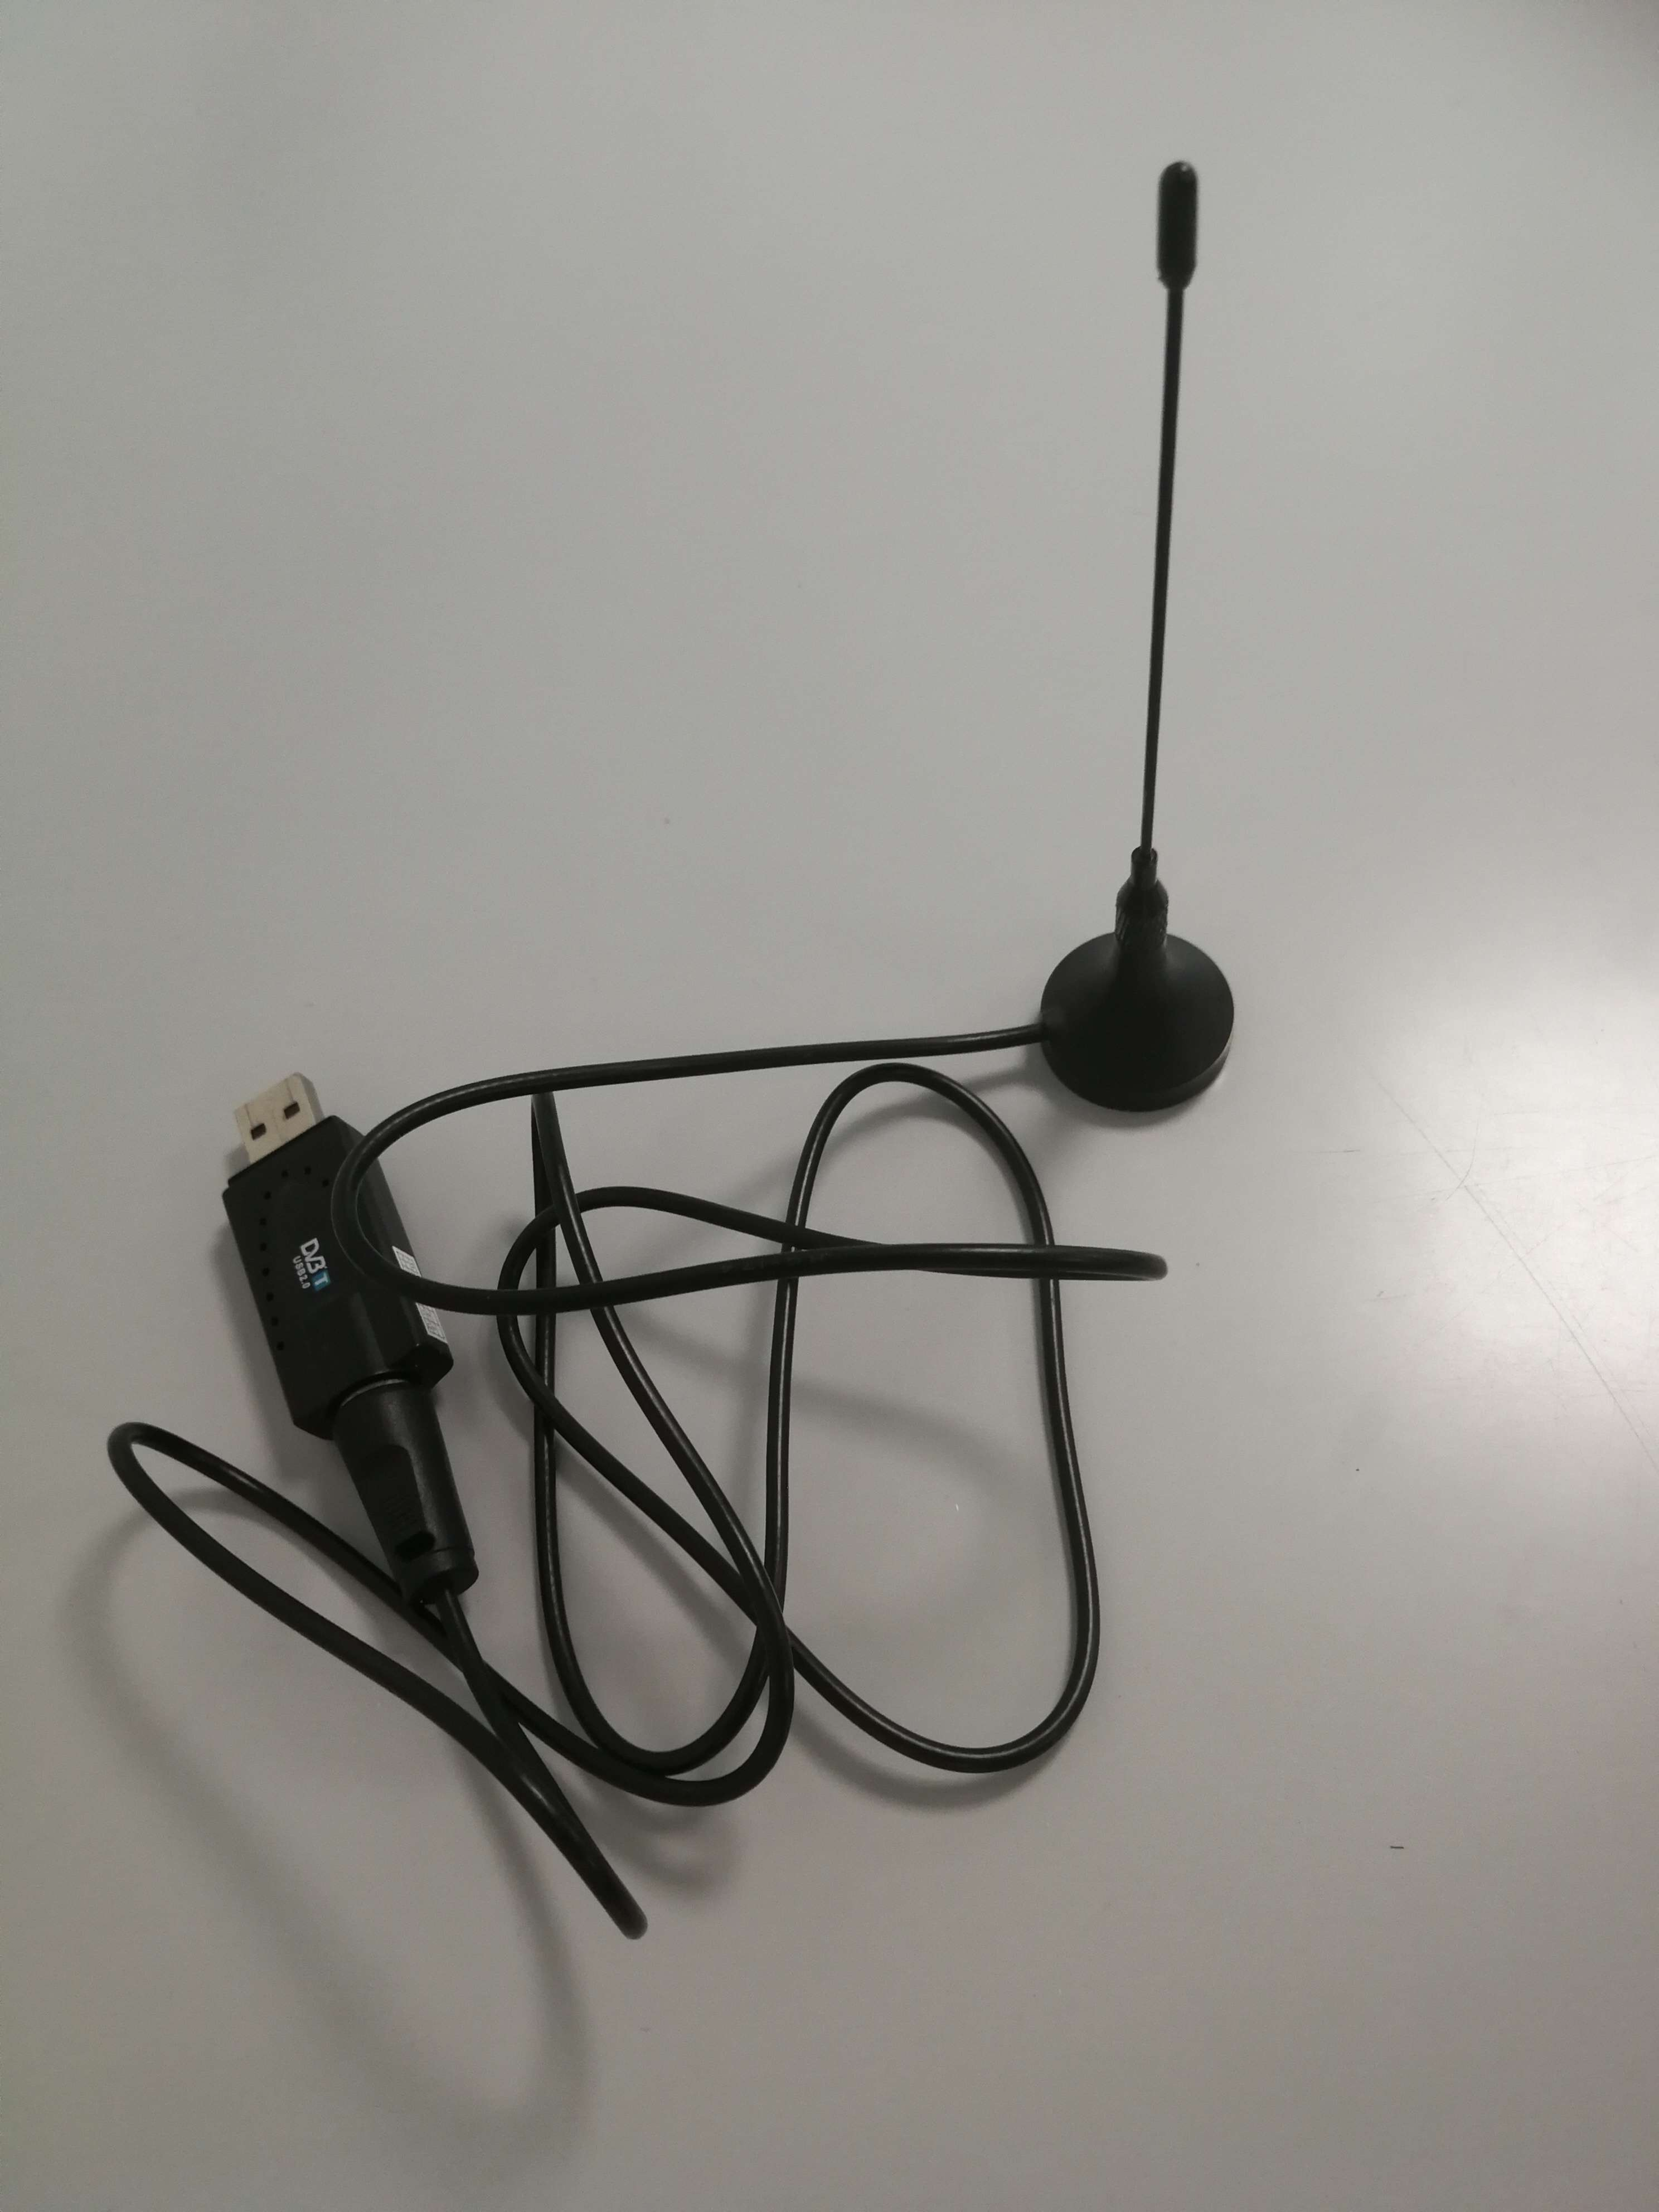
\includegraphics[scale=0.08]{images/dvbt.png}
\caption{RTL SDR Dvb-T dongle}\label{term31}
\end{figure}

\newpage

\subsubsection{RTL-SDR R820T2}

La deuxième radio logicielle utilisée est la RTL SDR R820T2. Il y a deux différence majeures avec la radio dvb-t. L'antenne de cette radio logicielle est de meilleure qualité. Le tuner chip de cette sdr est un r820t2 tuner. Cette version est une version améliorée du tuner qui se trouve dans la dvb-t, ce qui a pour impact une réduction du bruit, une meilleur sensibilité et une couverturee de fréquence plus large. La figure \ref{term32} montre la sdr utilisée.


\begin{figure}[h]
\centering

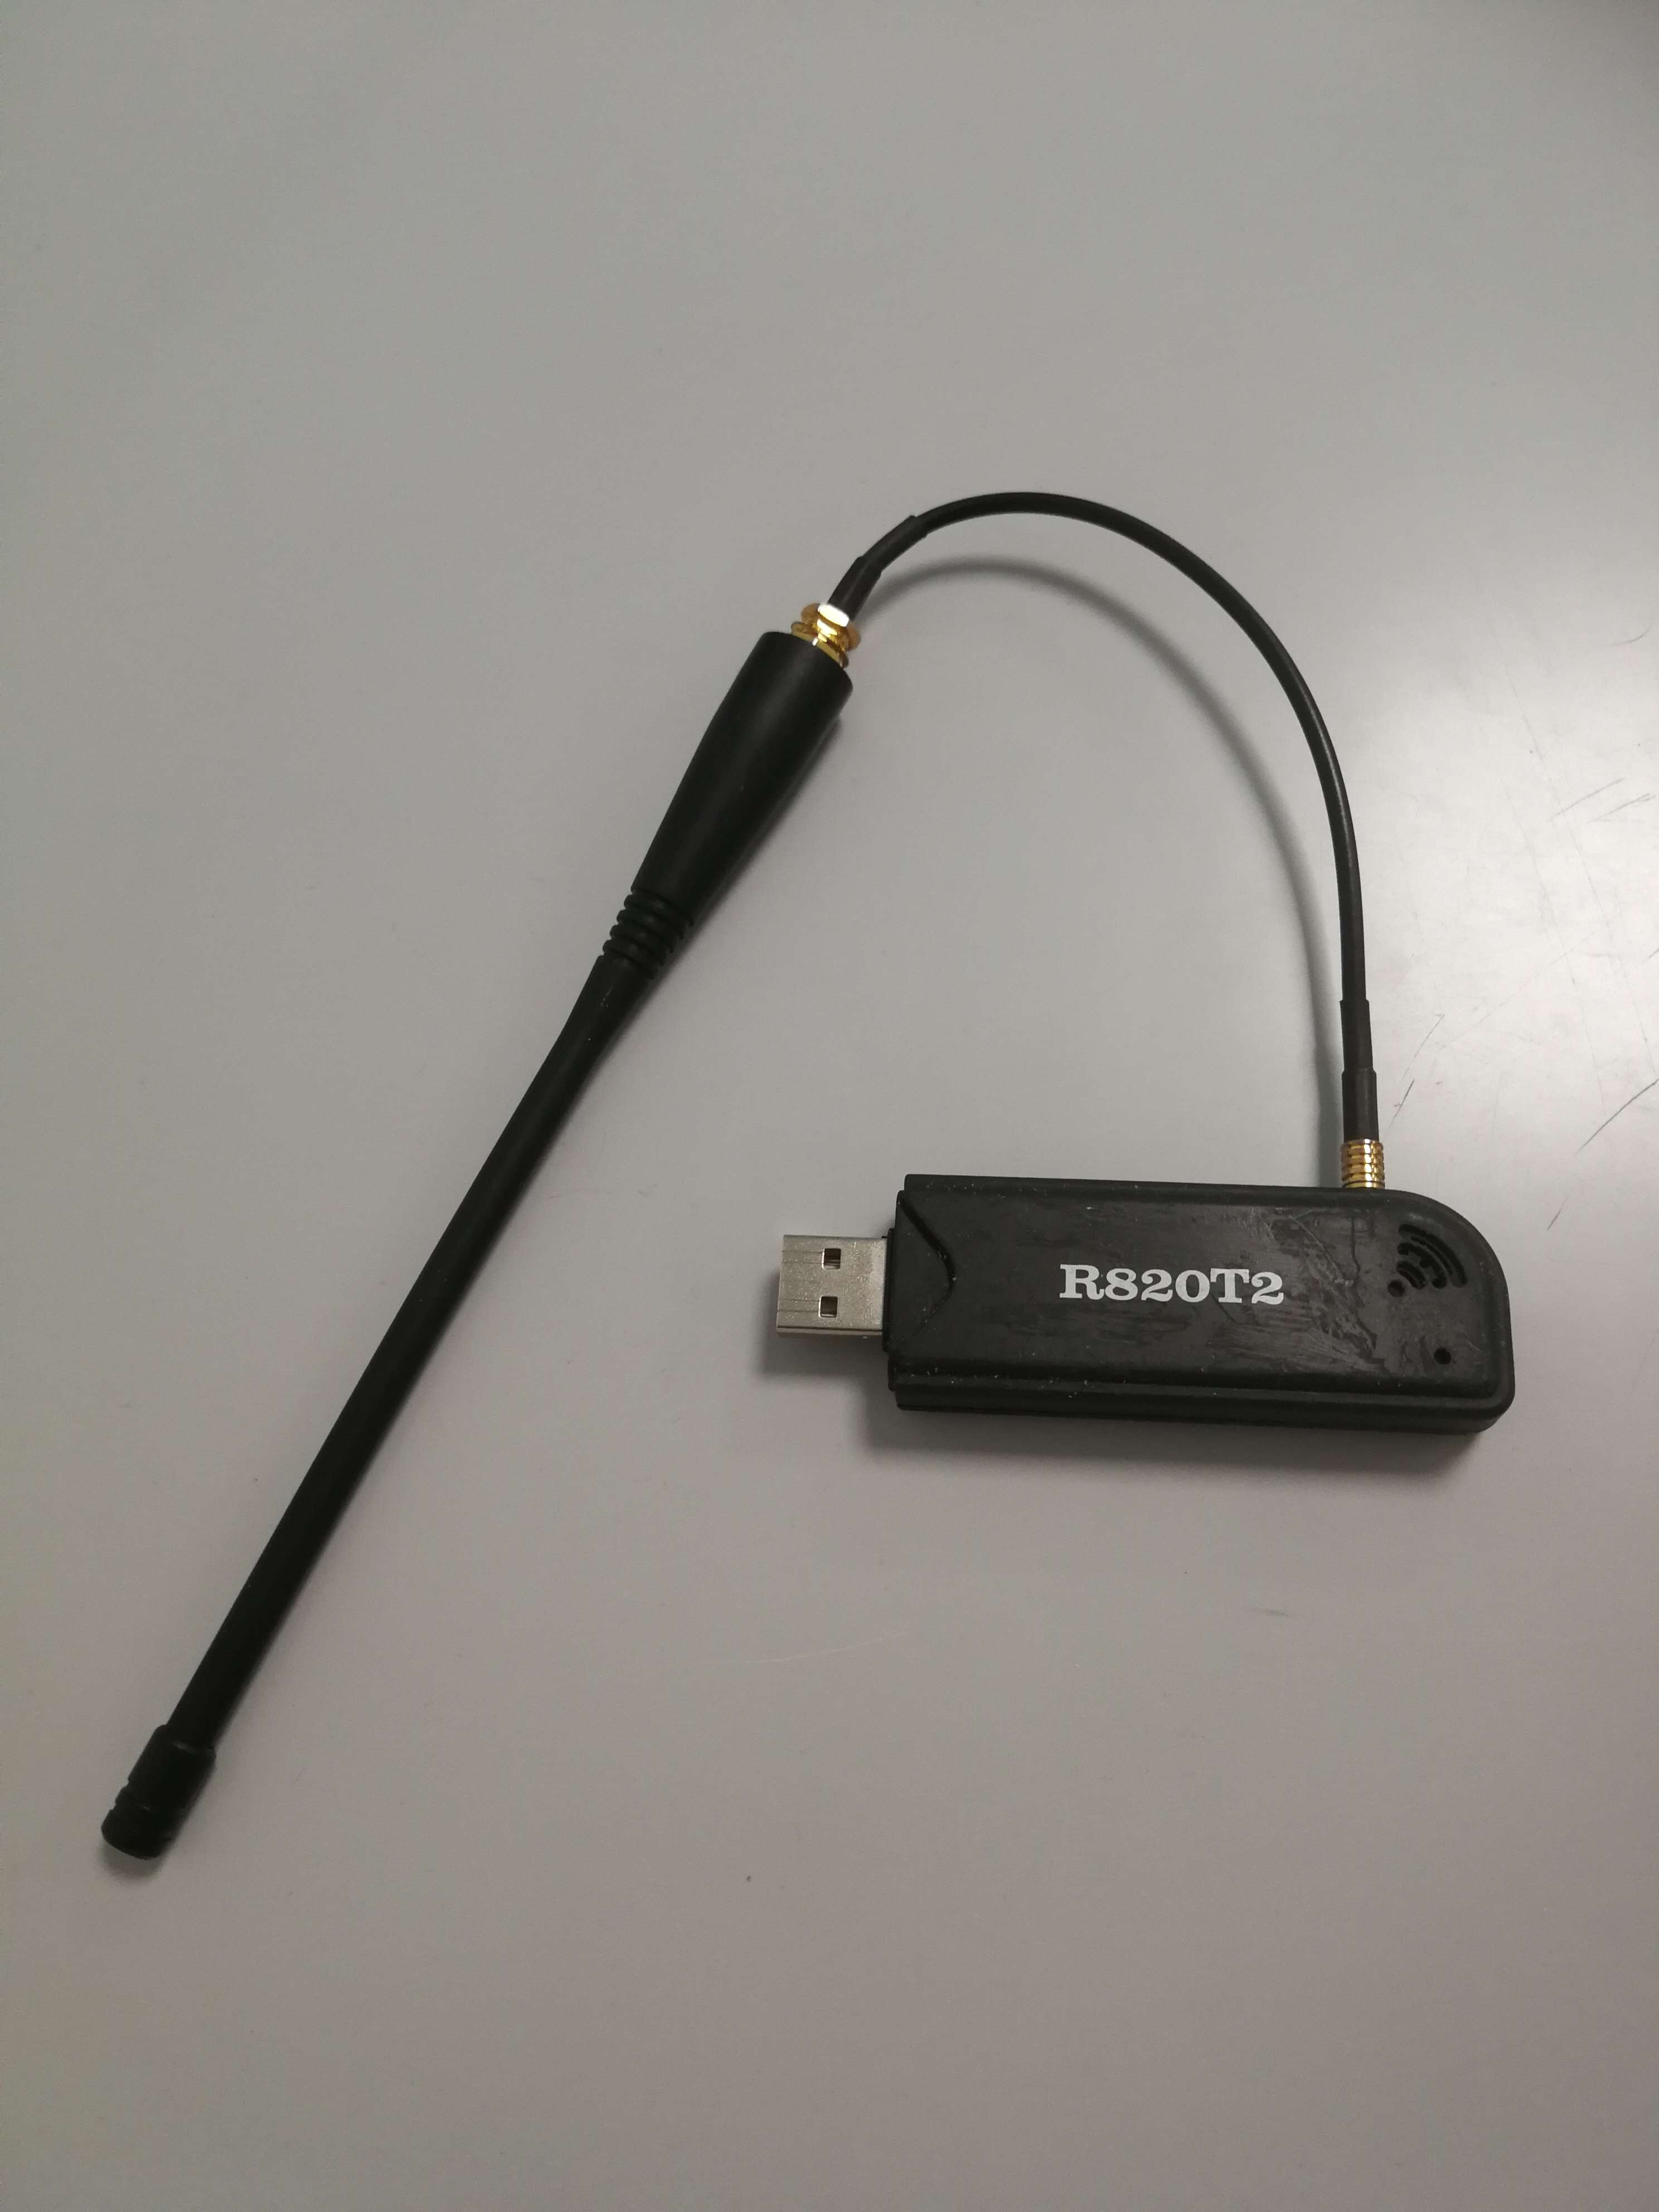
\includegraphics[scale=0.08]{images/r820t2.png}
\caption{RTL SDR R820T2}\label{term32}
\end{figure}

\newpage


\subsubsection{HackRf One}

La dernière radio logicielle utilisée est la HackRf one. Au dela du prix, cette dernière radio est différente des deux autres. Elle est notament capable de gérer la transmission et la réception de signaux, là ou les deux autres sont uniquement des récepteurs. Si la rtl sdr r820t2 offrait déja une qualité de signal supérieureà la dvb-t, celui de la hack rf est encore plus net. La figure \ref{fig:both_images} montre la sdr hackRf avec l'antenne utilisée posée sur un trepied.

\begin{figure}[h]
\centering
\begin{subfigure}{0.4\textwidth}
  \centering
  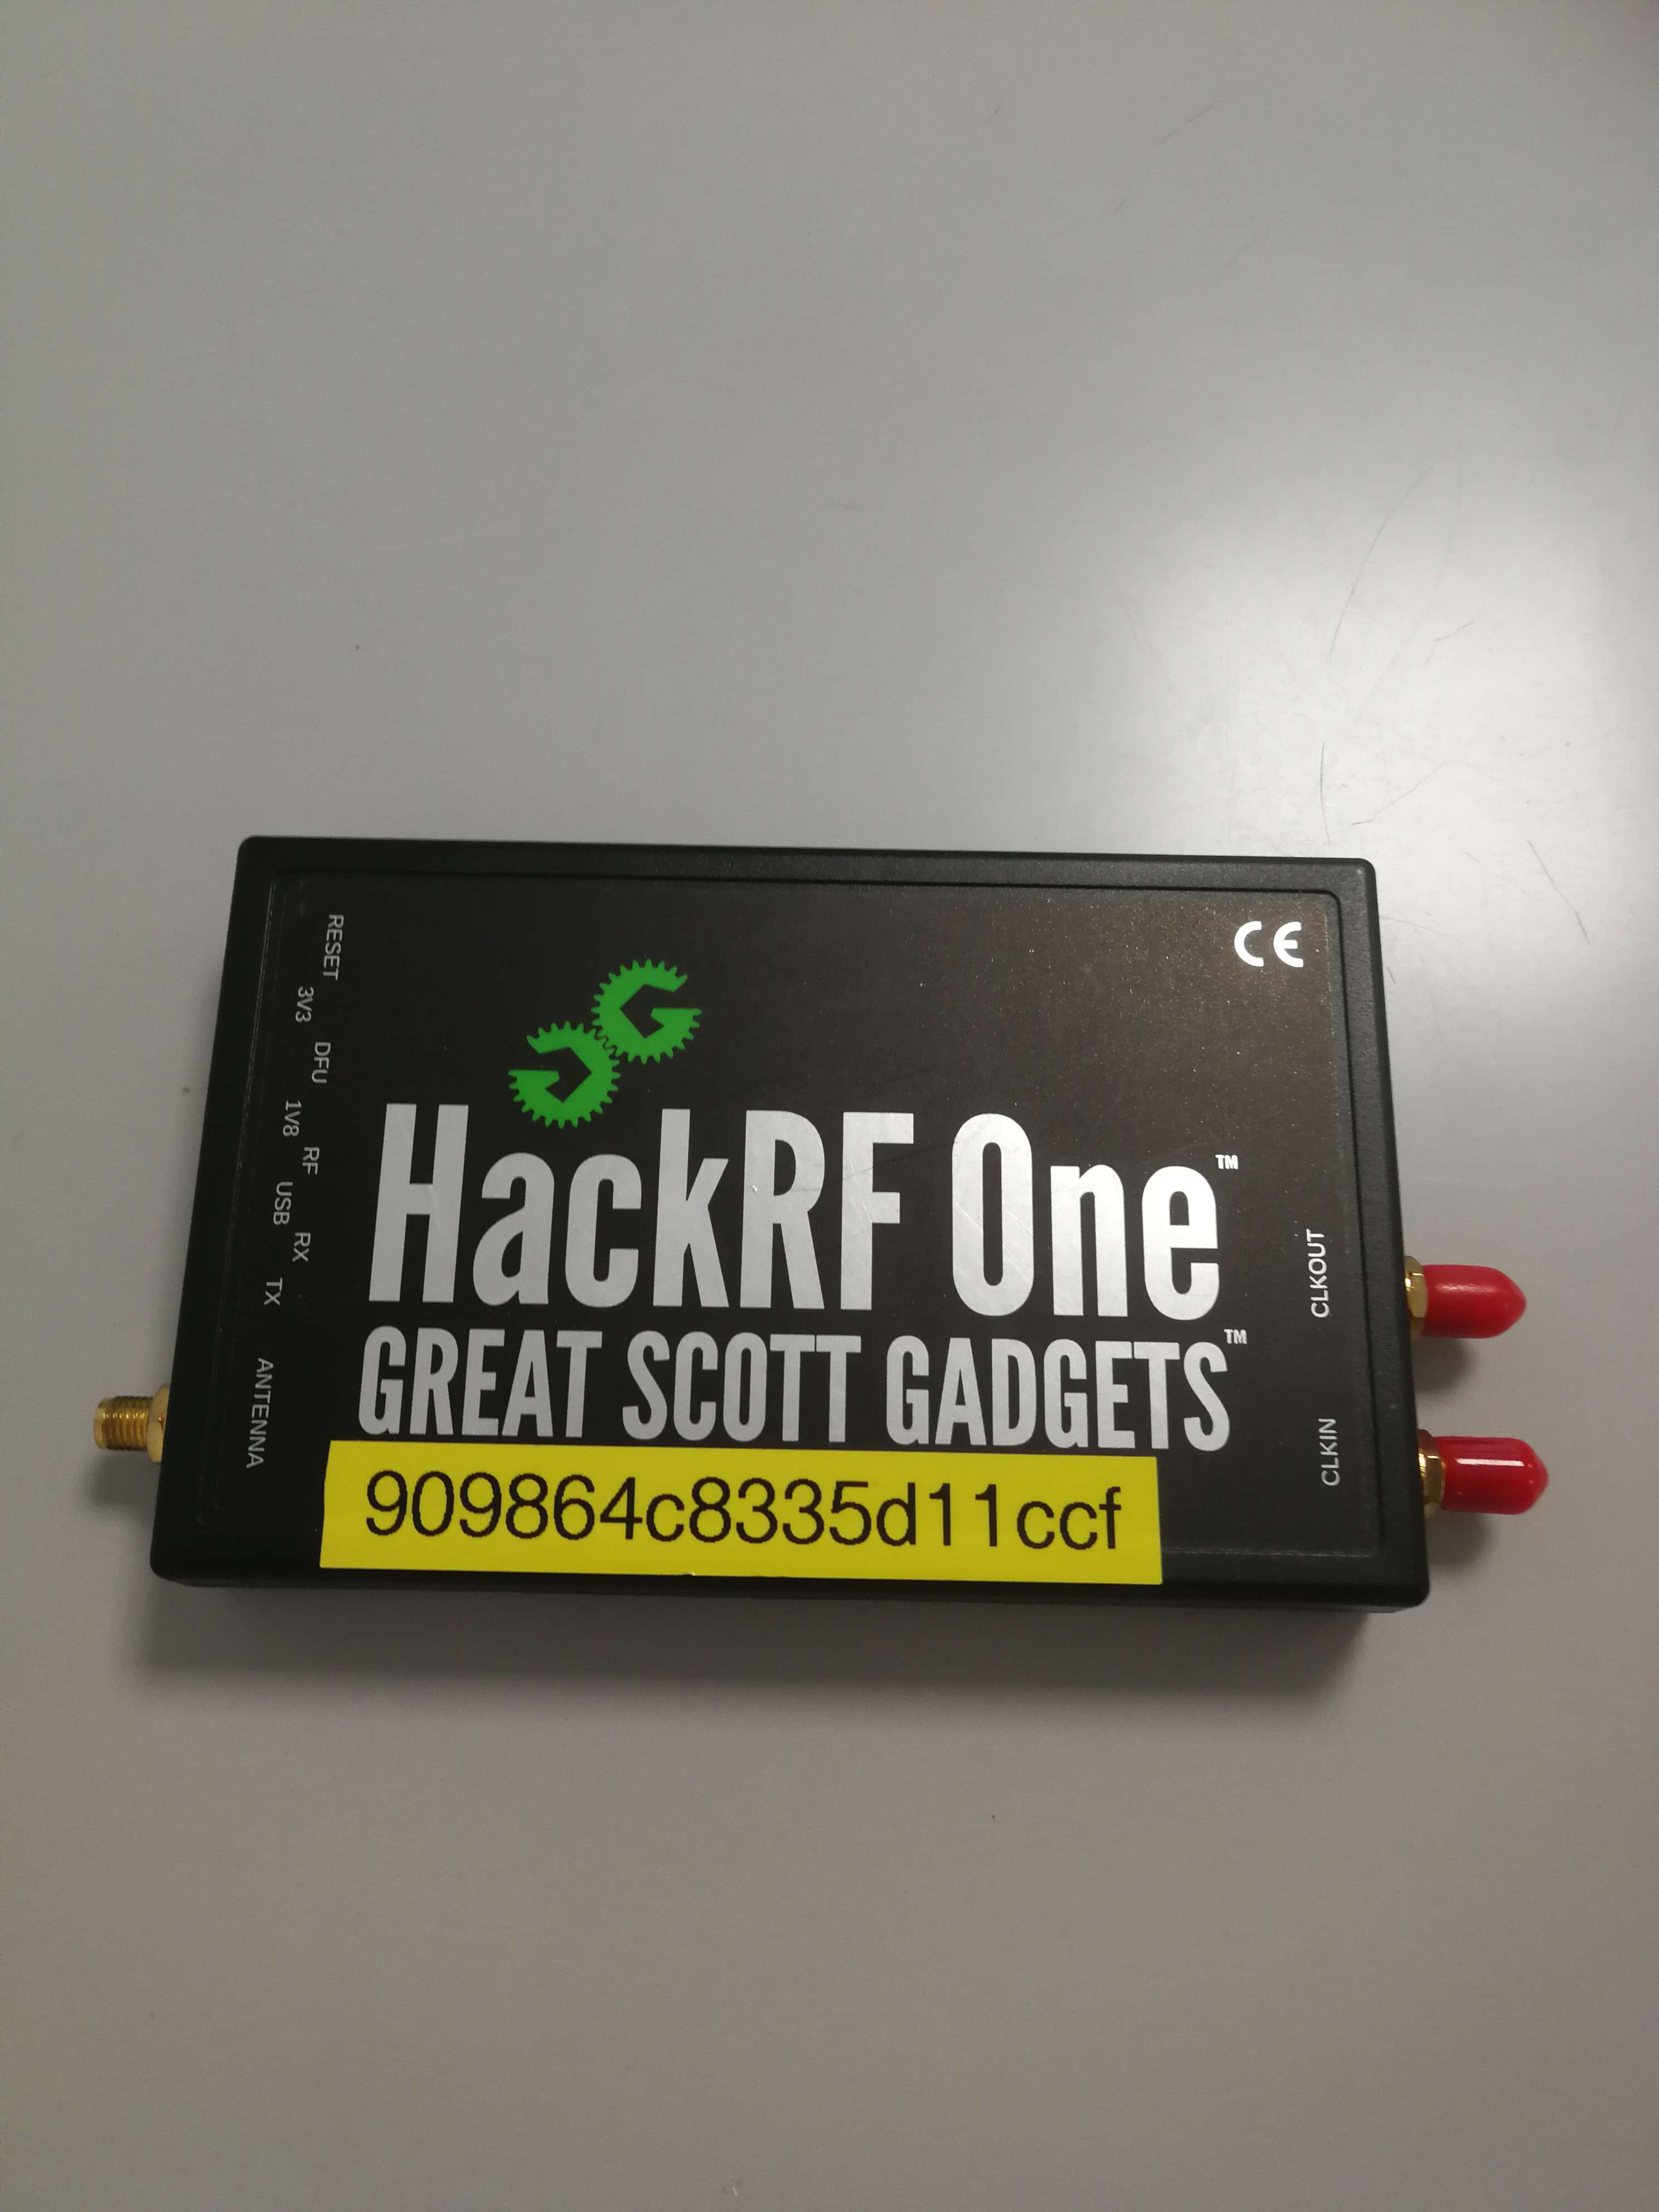
\includegraphics[width=\textwidth]{images/hackrf.png}
  \caption{SDR HackRF One}
  \label{term330}
\end{subfigure}
\hspace{0.5cm} % Adjust the horizontal space between the subfigures
\begin{subfigure}{0.4\textwidth}
  \centering
  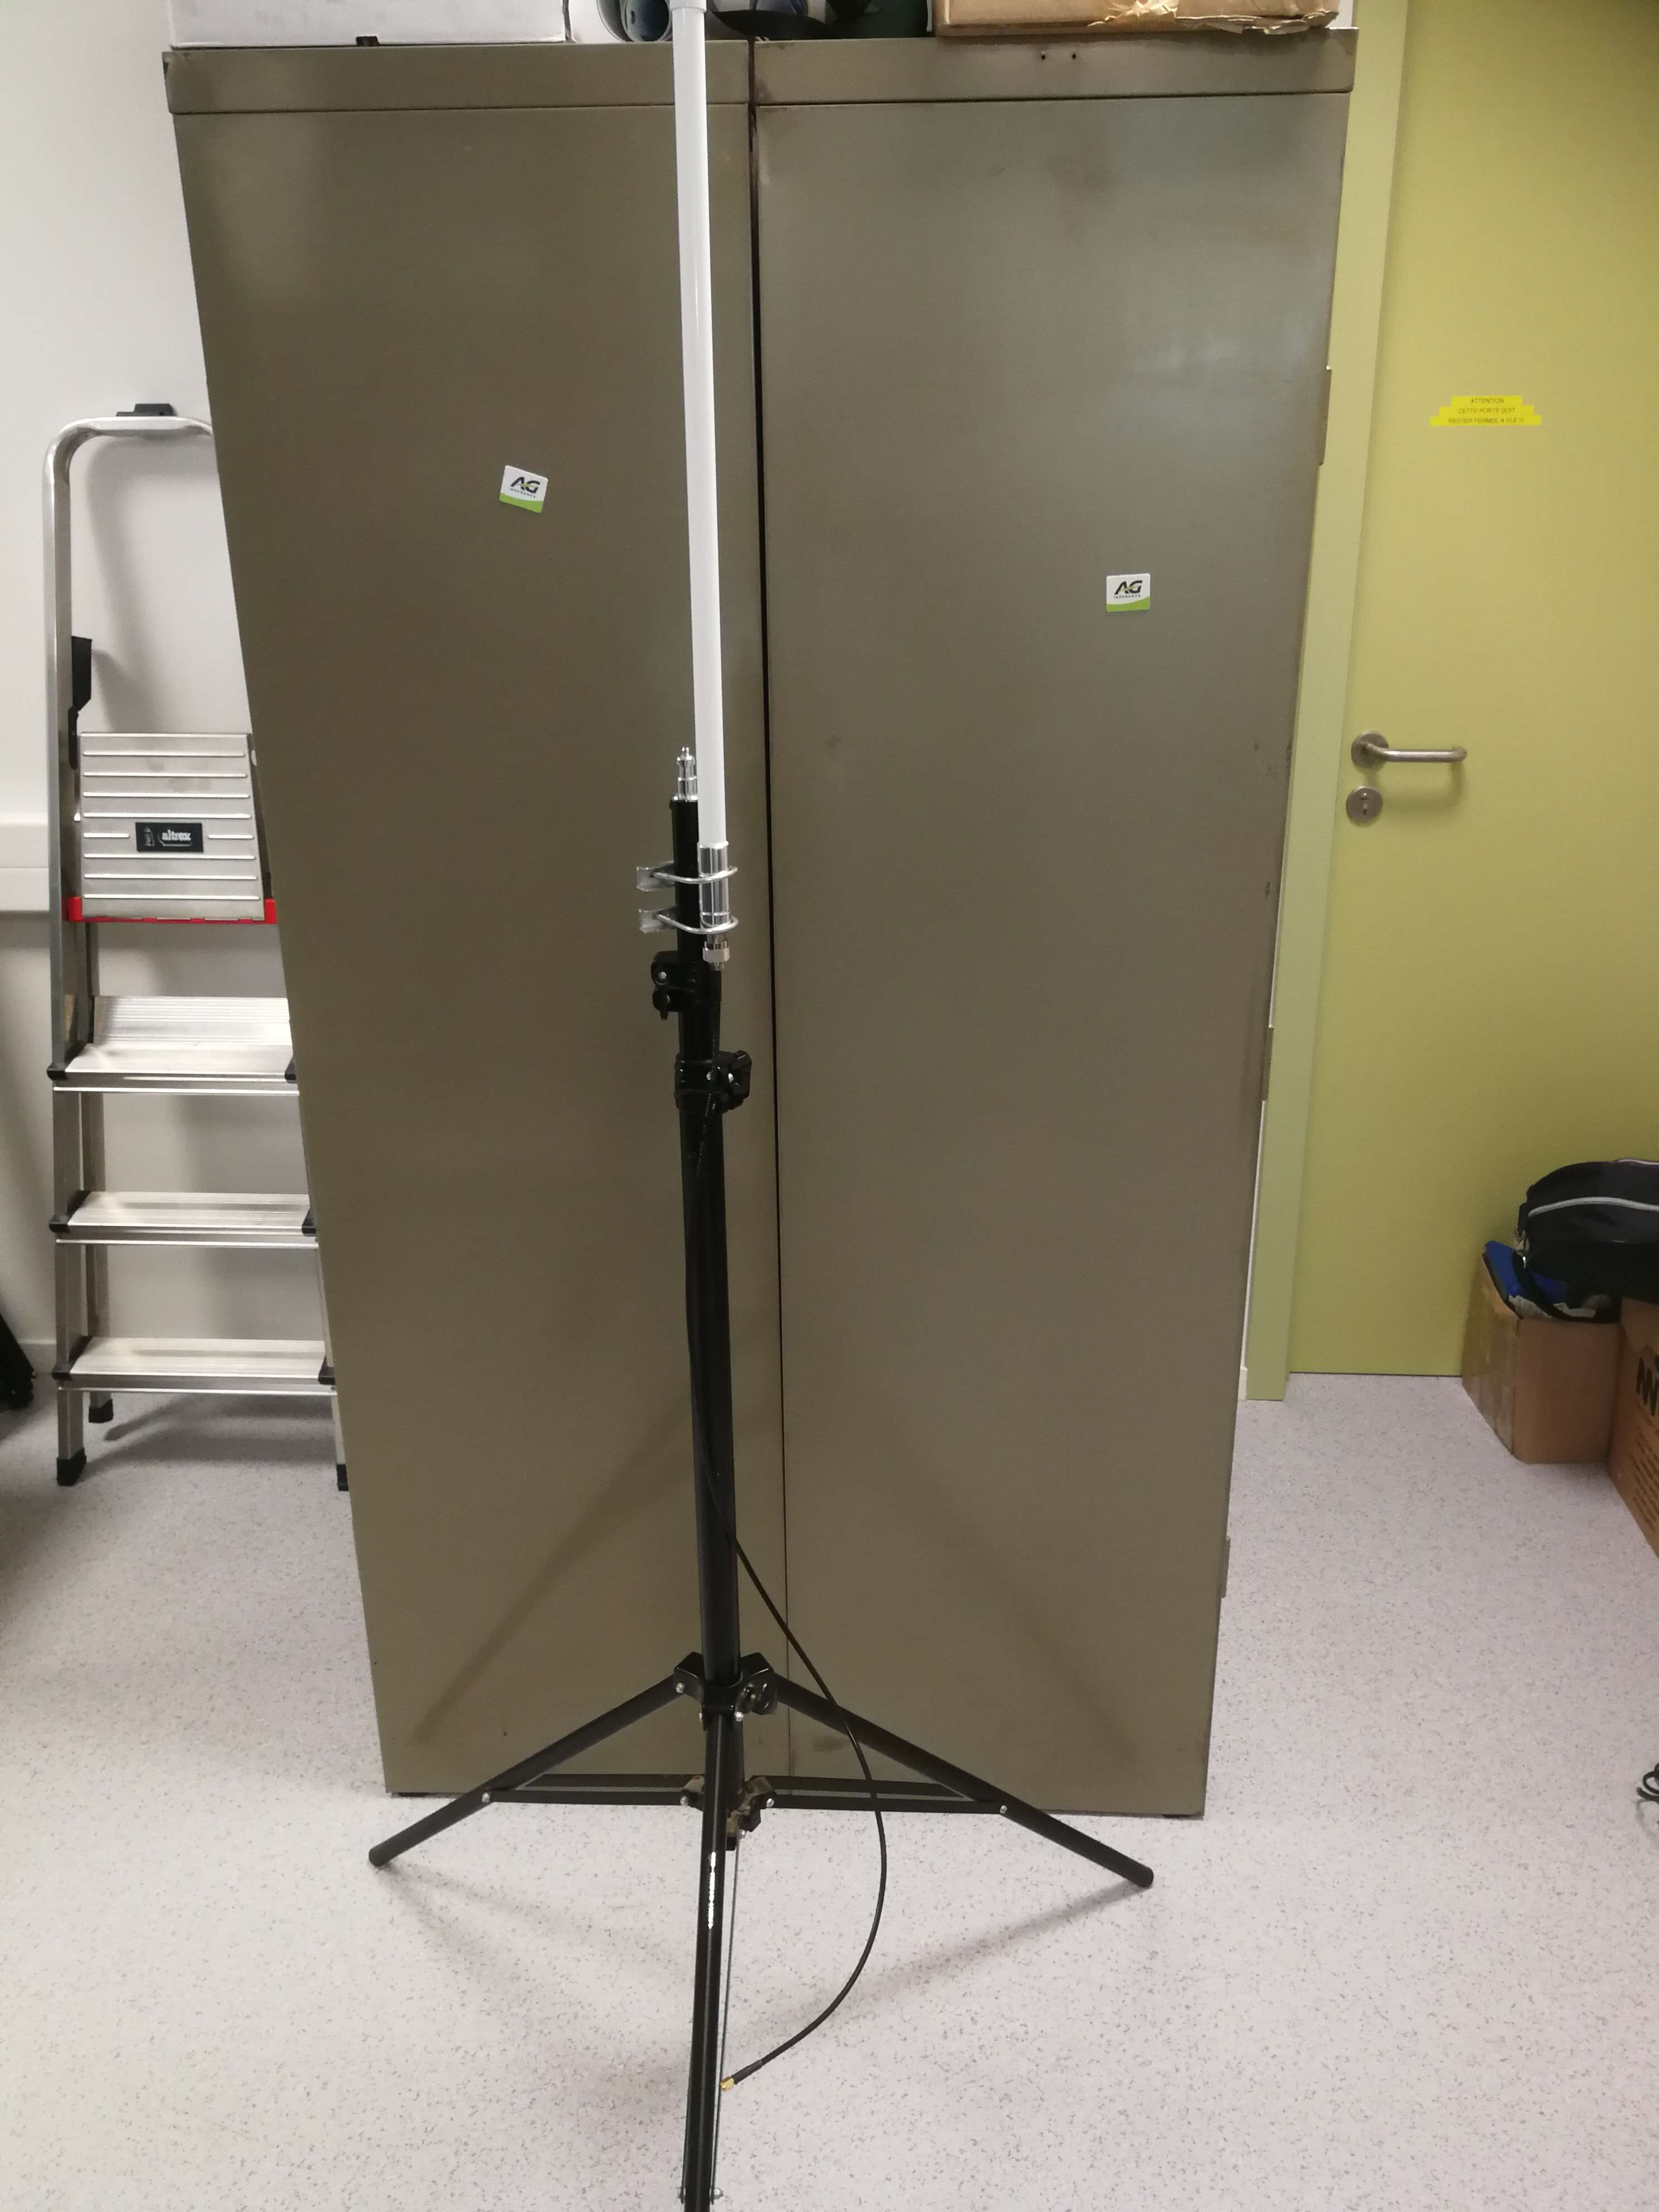
\includegraphics[width=\textwidth]{images/pied.png}
  \caption{Antenne}
  \label{term340}
\end{subfigure}
\caption{SDR HackRf One avec son antenne}
\label{fig:both_images}
\end{figure}

\newpage

\newpage

\subsection{Module d'émission Lora}

\subsubsection{module RN2483}

\begin{figure}[h]
\centering

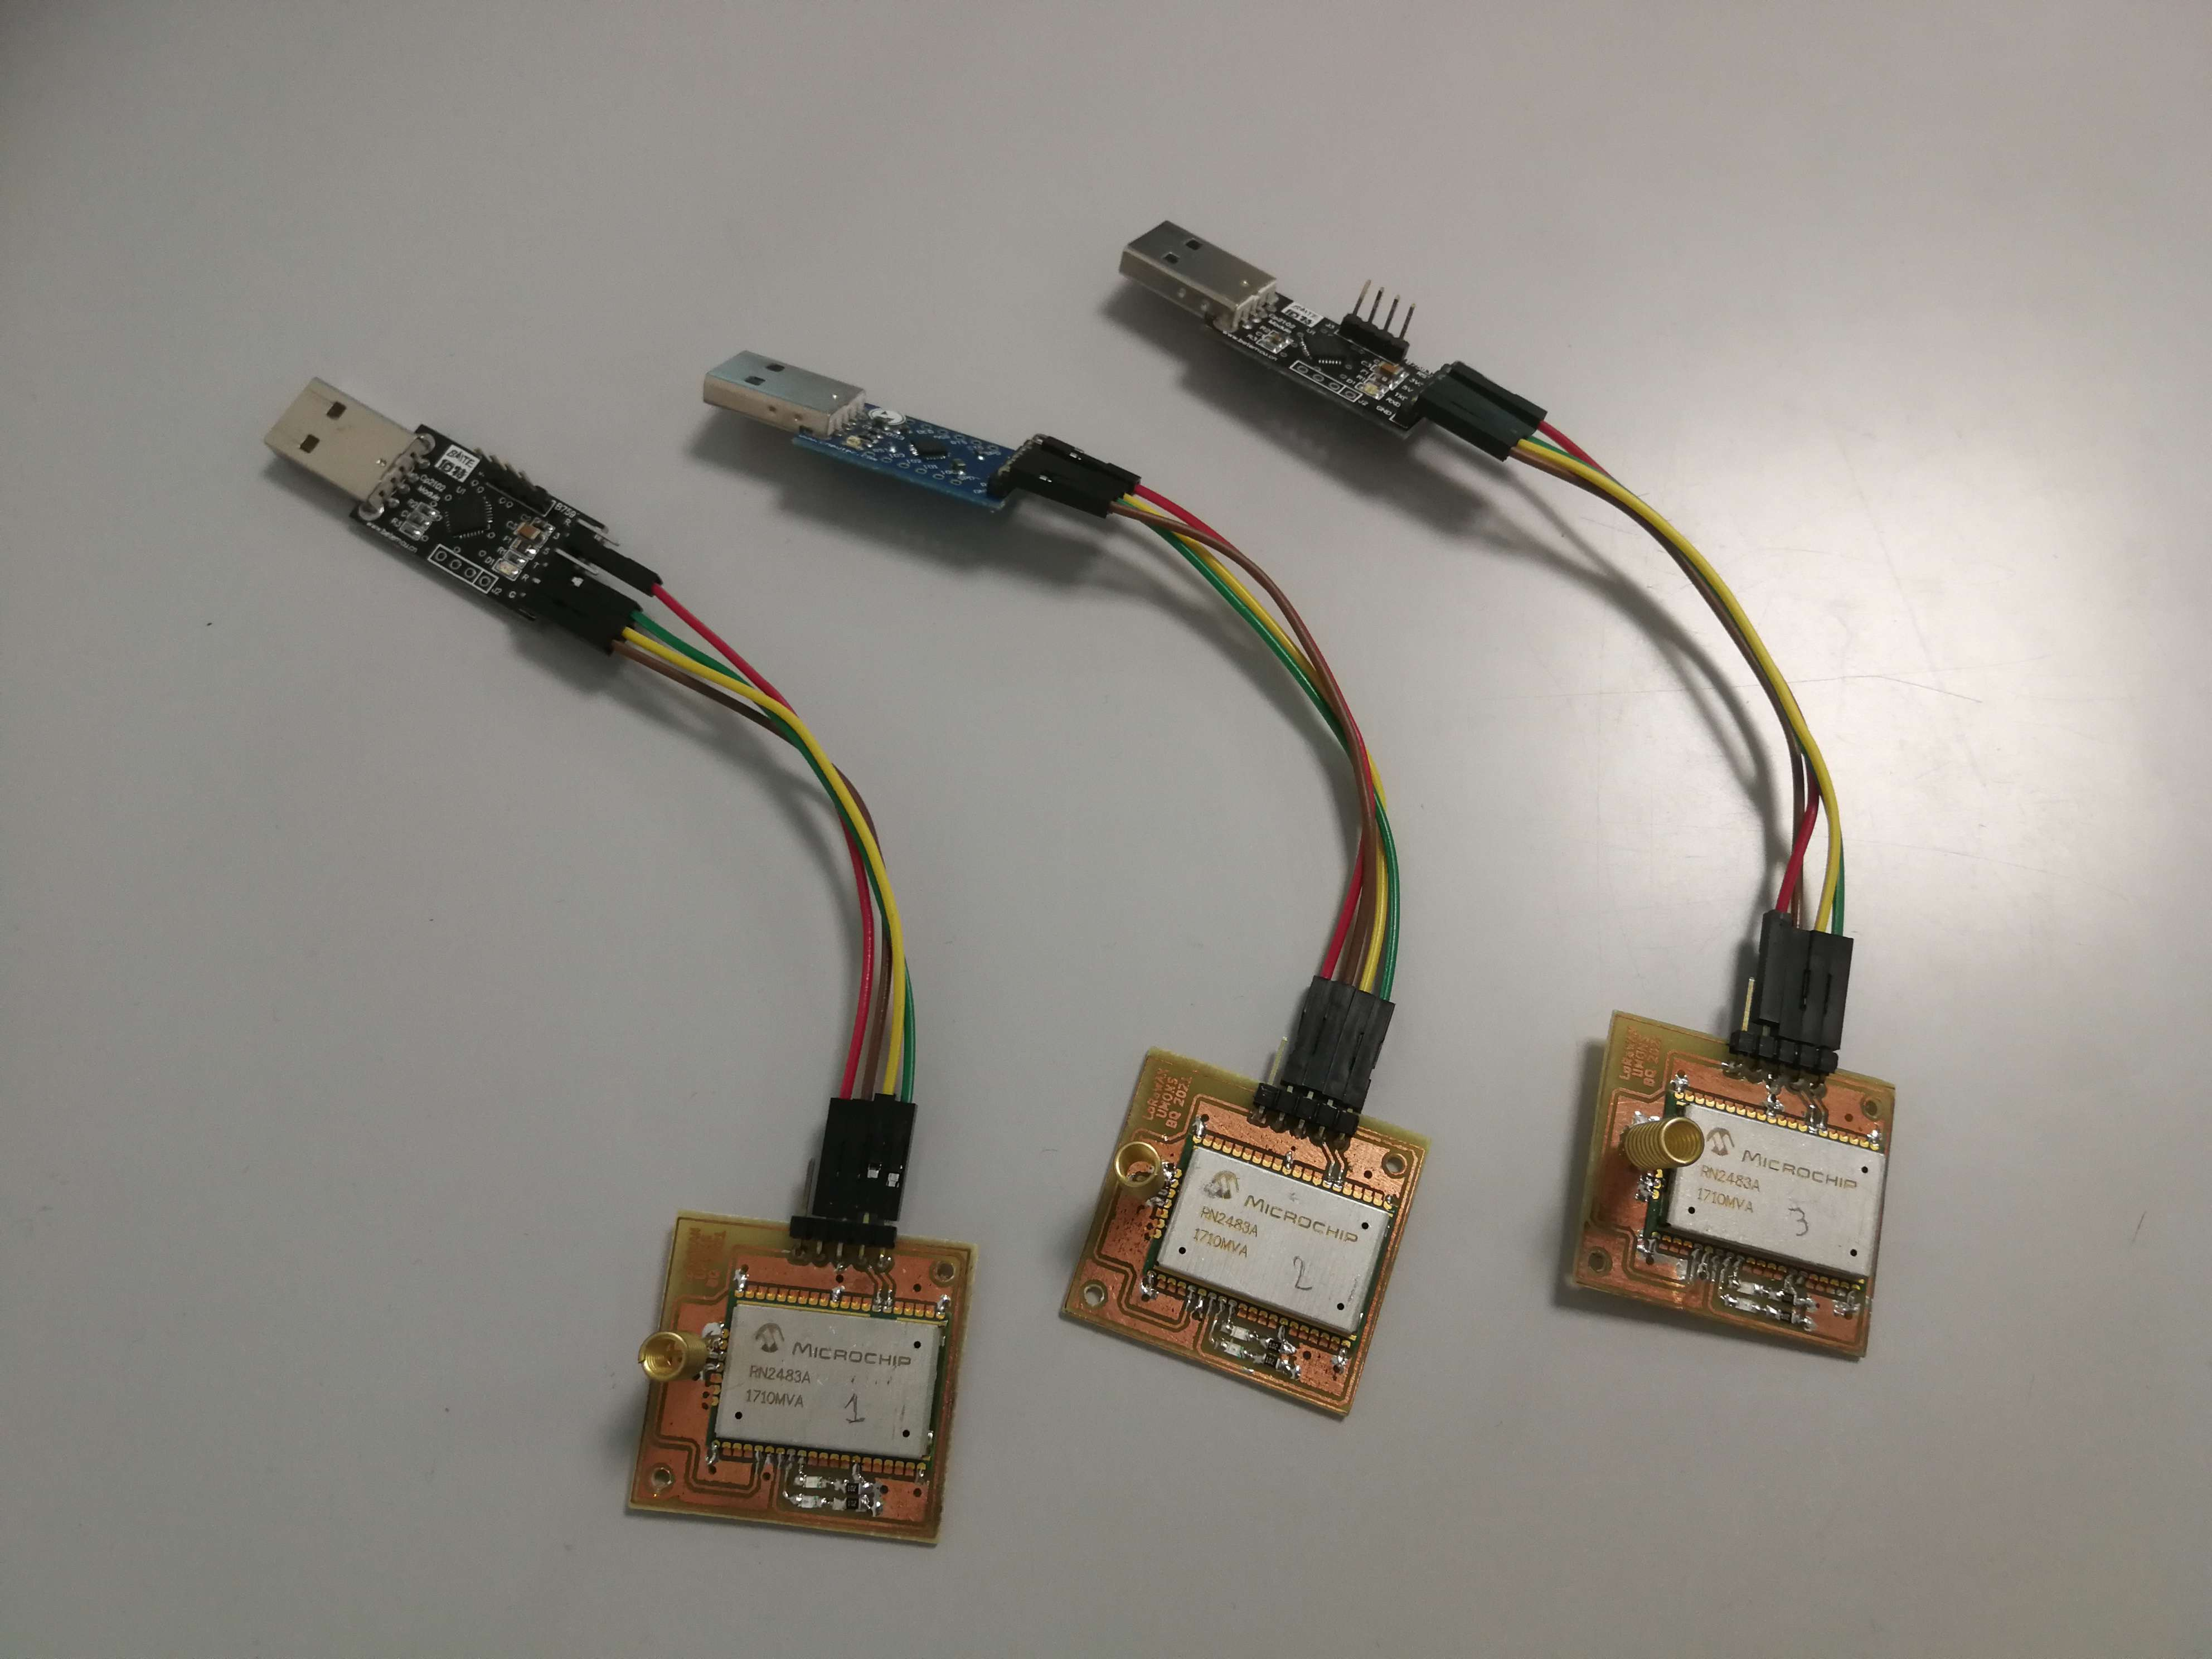
\includegraphics[scale=0.08]{images/rn2483.png}
\caption{3 modules RN2483}\label{term34}
\end{figure}


Le microchip RN2483 est un module de technologie spécifique à LoRa. Bien que Microchip soit une compagnie qui produit de nombreux microcontrolleur, cet appareil n'en est pas un. Le module rn2483 de la figure \ref{term34} est un simple \textit{transceiver (transmitter and receiver)} radio permetant de communiquer à longue portée et à faible coup. La documentation sur cet appareil est disponible au lien suivant : (lien). 

Voici quelques spécificités sur le module:
\begin{itemize}
\item Il comprend la technologie de modulation LoRa, ce qui lui donne son atout de faibles consomation et longue portée. Il gère également les modulations \textit{FSK (frequency shift keying)} et \textit{GFSK (Gaussian frequency shift keying)}.
\item Une faible consomation induit une faible puissance, le module possède un amplificateur de puissance maximale de 14dBm.
\item Les bande de fréquences disponibles sont compatible avec la bande ISM. Le module couvre de 863Mhz à 870Mhz pour la région Européenne.
\item La data rate maximum en modulant avec LoRa est de 10937 bps (bit par seconde).
\item tous les paramètres TX sont configurables.
\end{itemize}

L'utilisation du module RN2483 est détaillée dans la section \ref{signallora}.

\subsubsection{pycom lopy}

\begin{figure}[h]
\centering

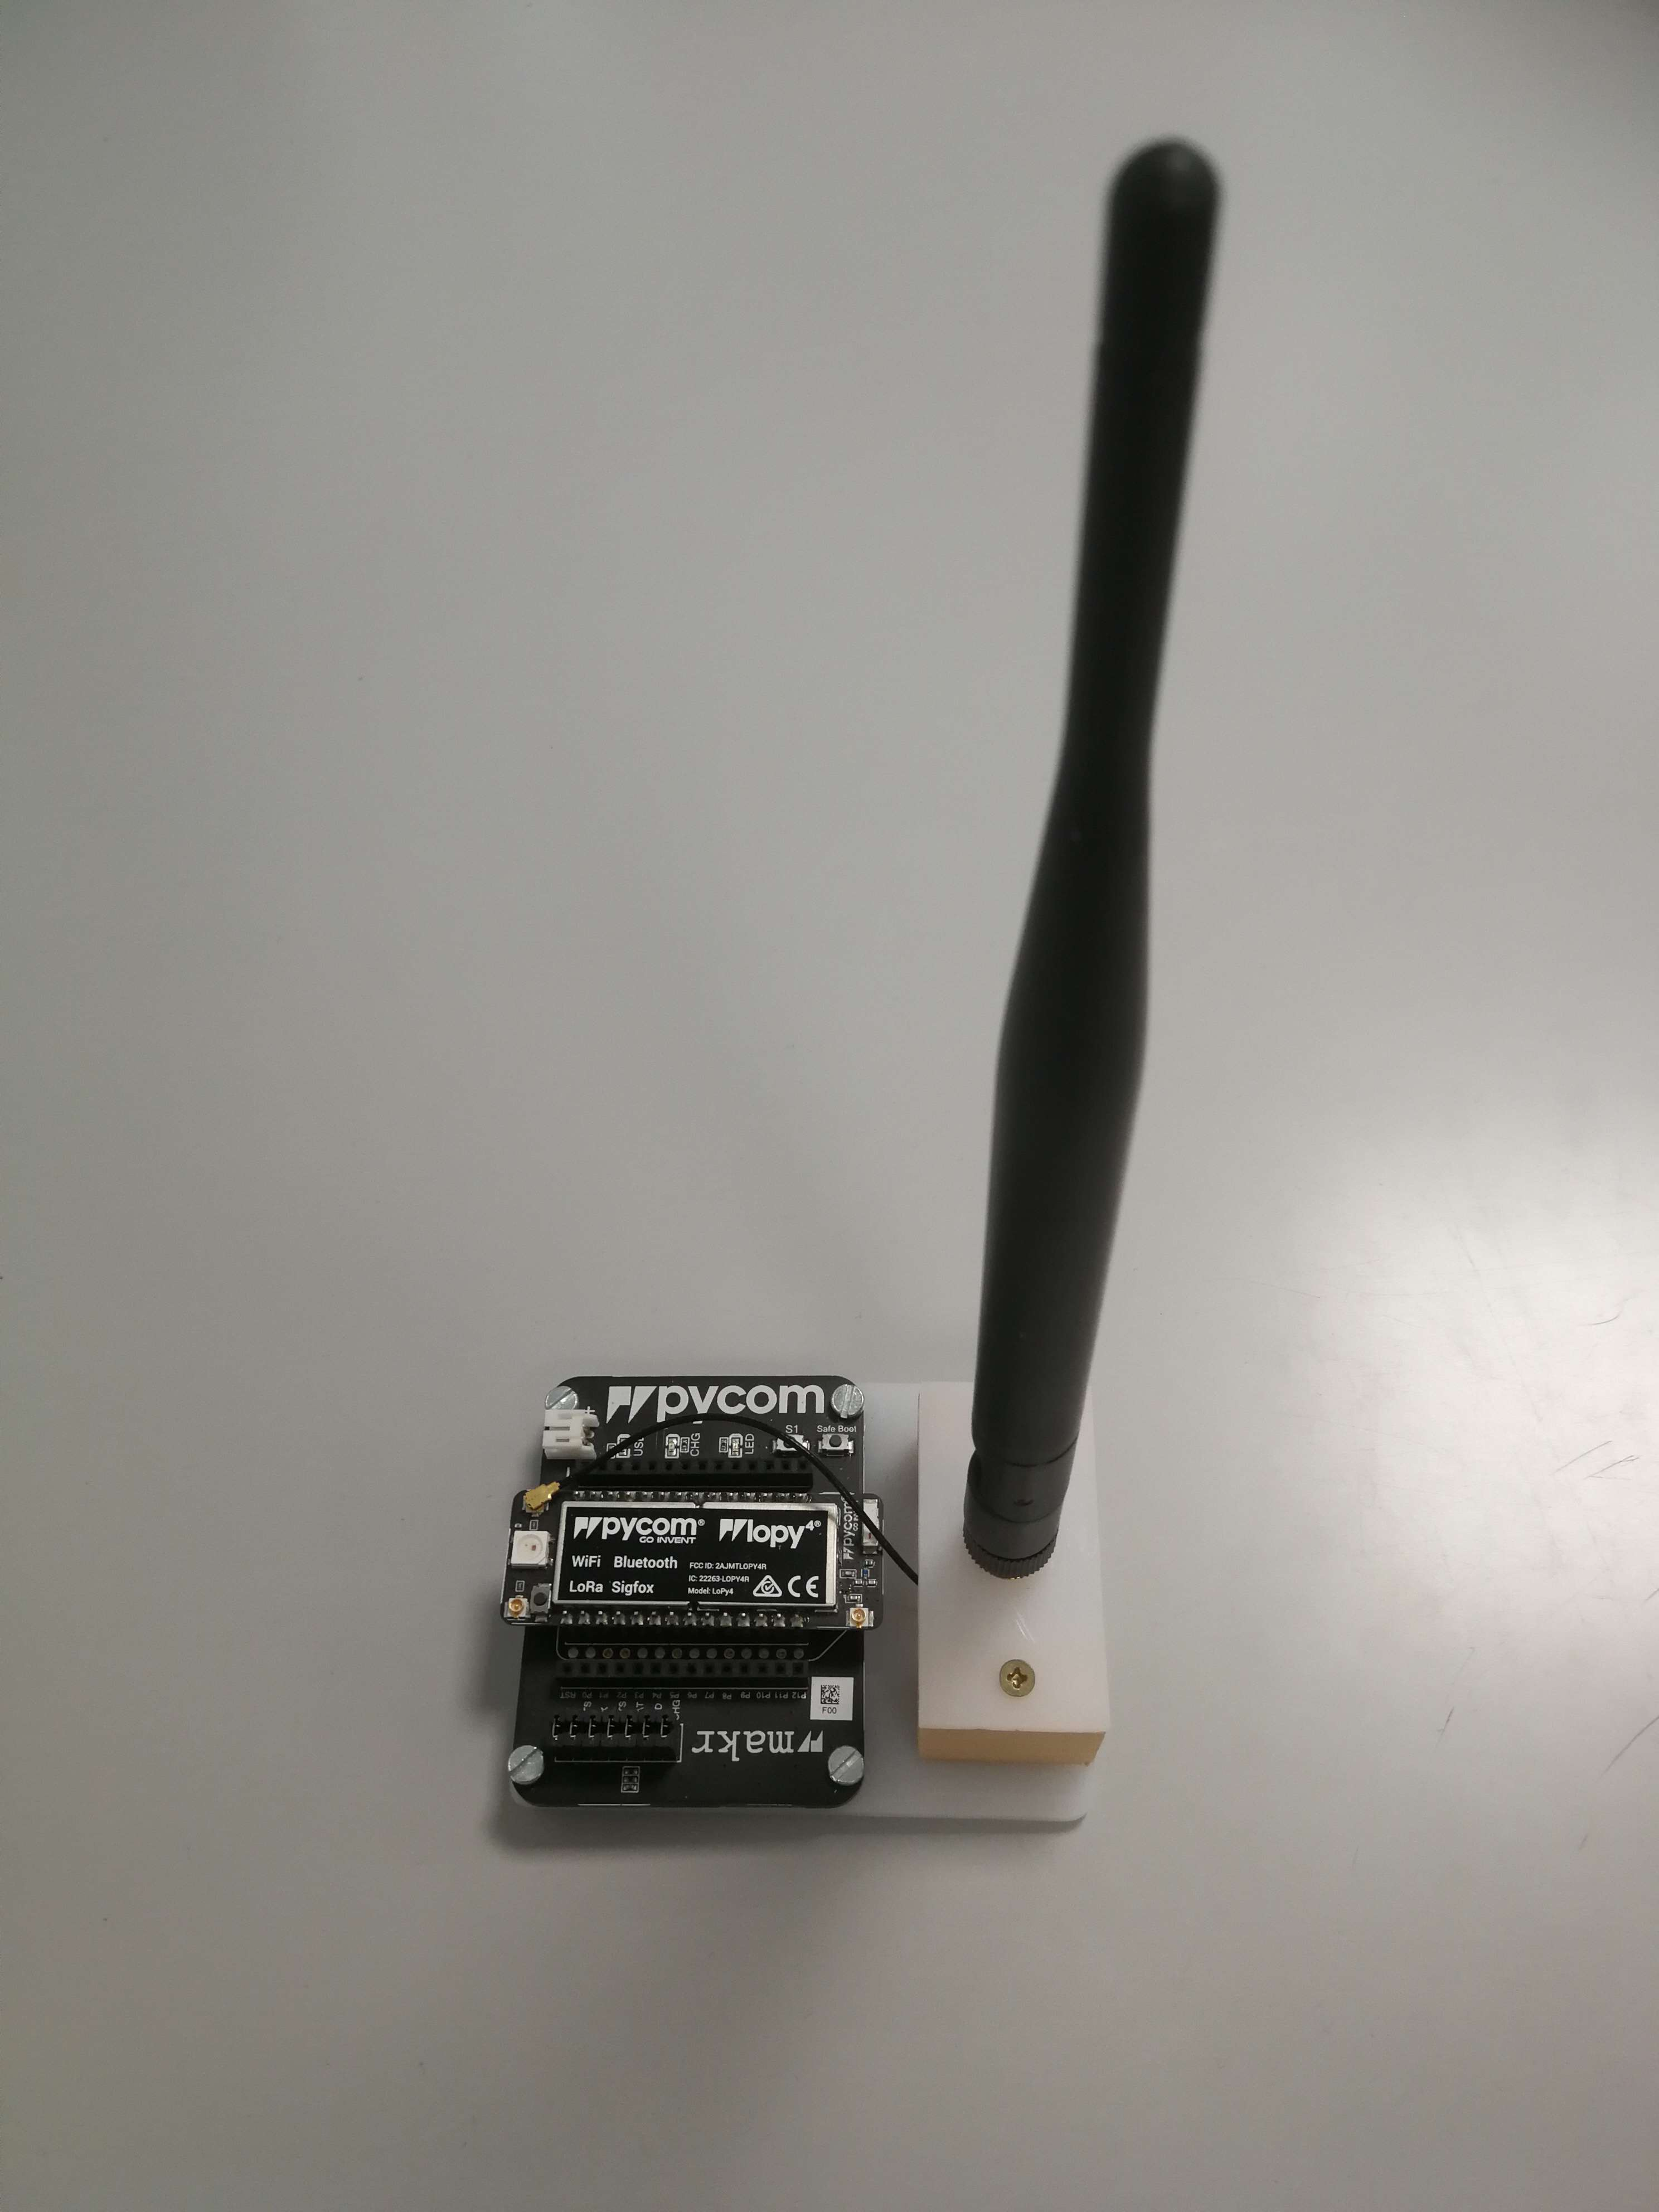
\includegraphics[scale=0.08]{images/lopy.png}
\caption{Un module Pycom Lopy avec une antenne}\label{term35}
\end{figure}

Ce module pycom est est appareil programmable en micro python, comprenant un microcontrolleur ainsi qu'une série de pins digitaux input/output,  des composantes de connectivité sans fil et un port micro USB. La figure \ref{term35} montre le module pycom connecté à une antenne.

\subsubsection{module arduino}\label{arduino}

\begin{figure}[h]
\centering

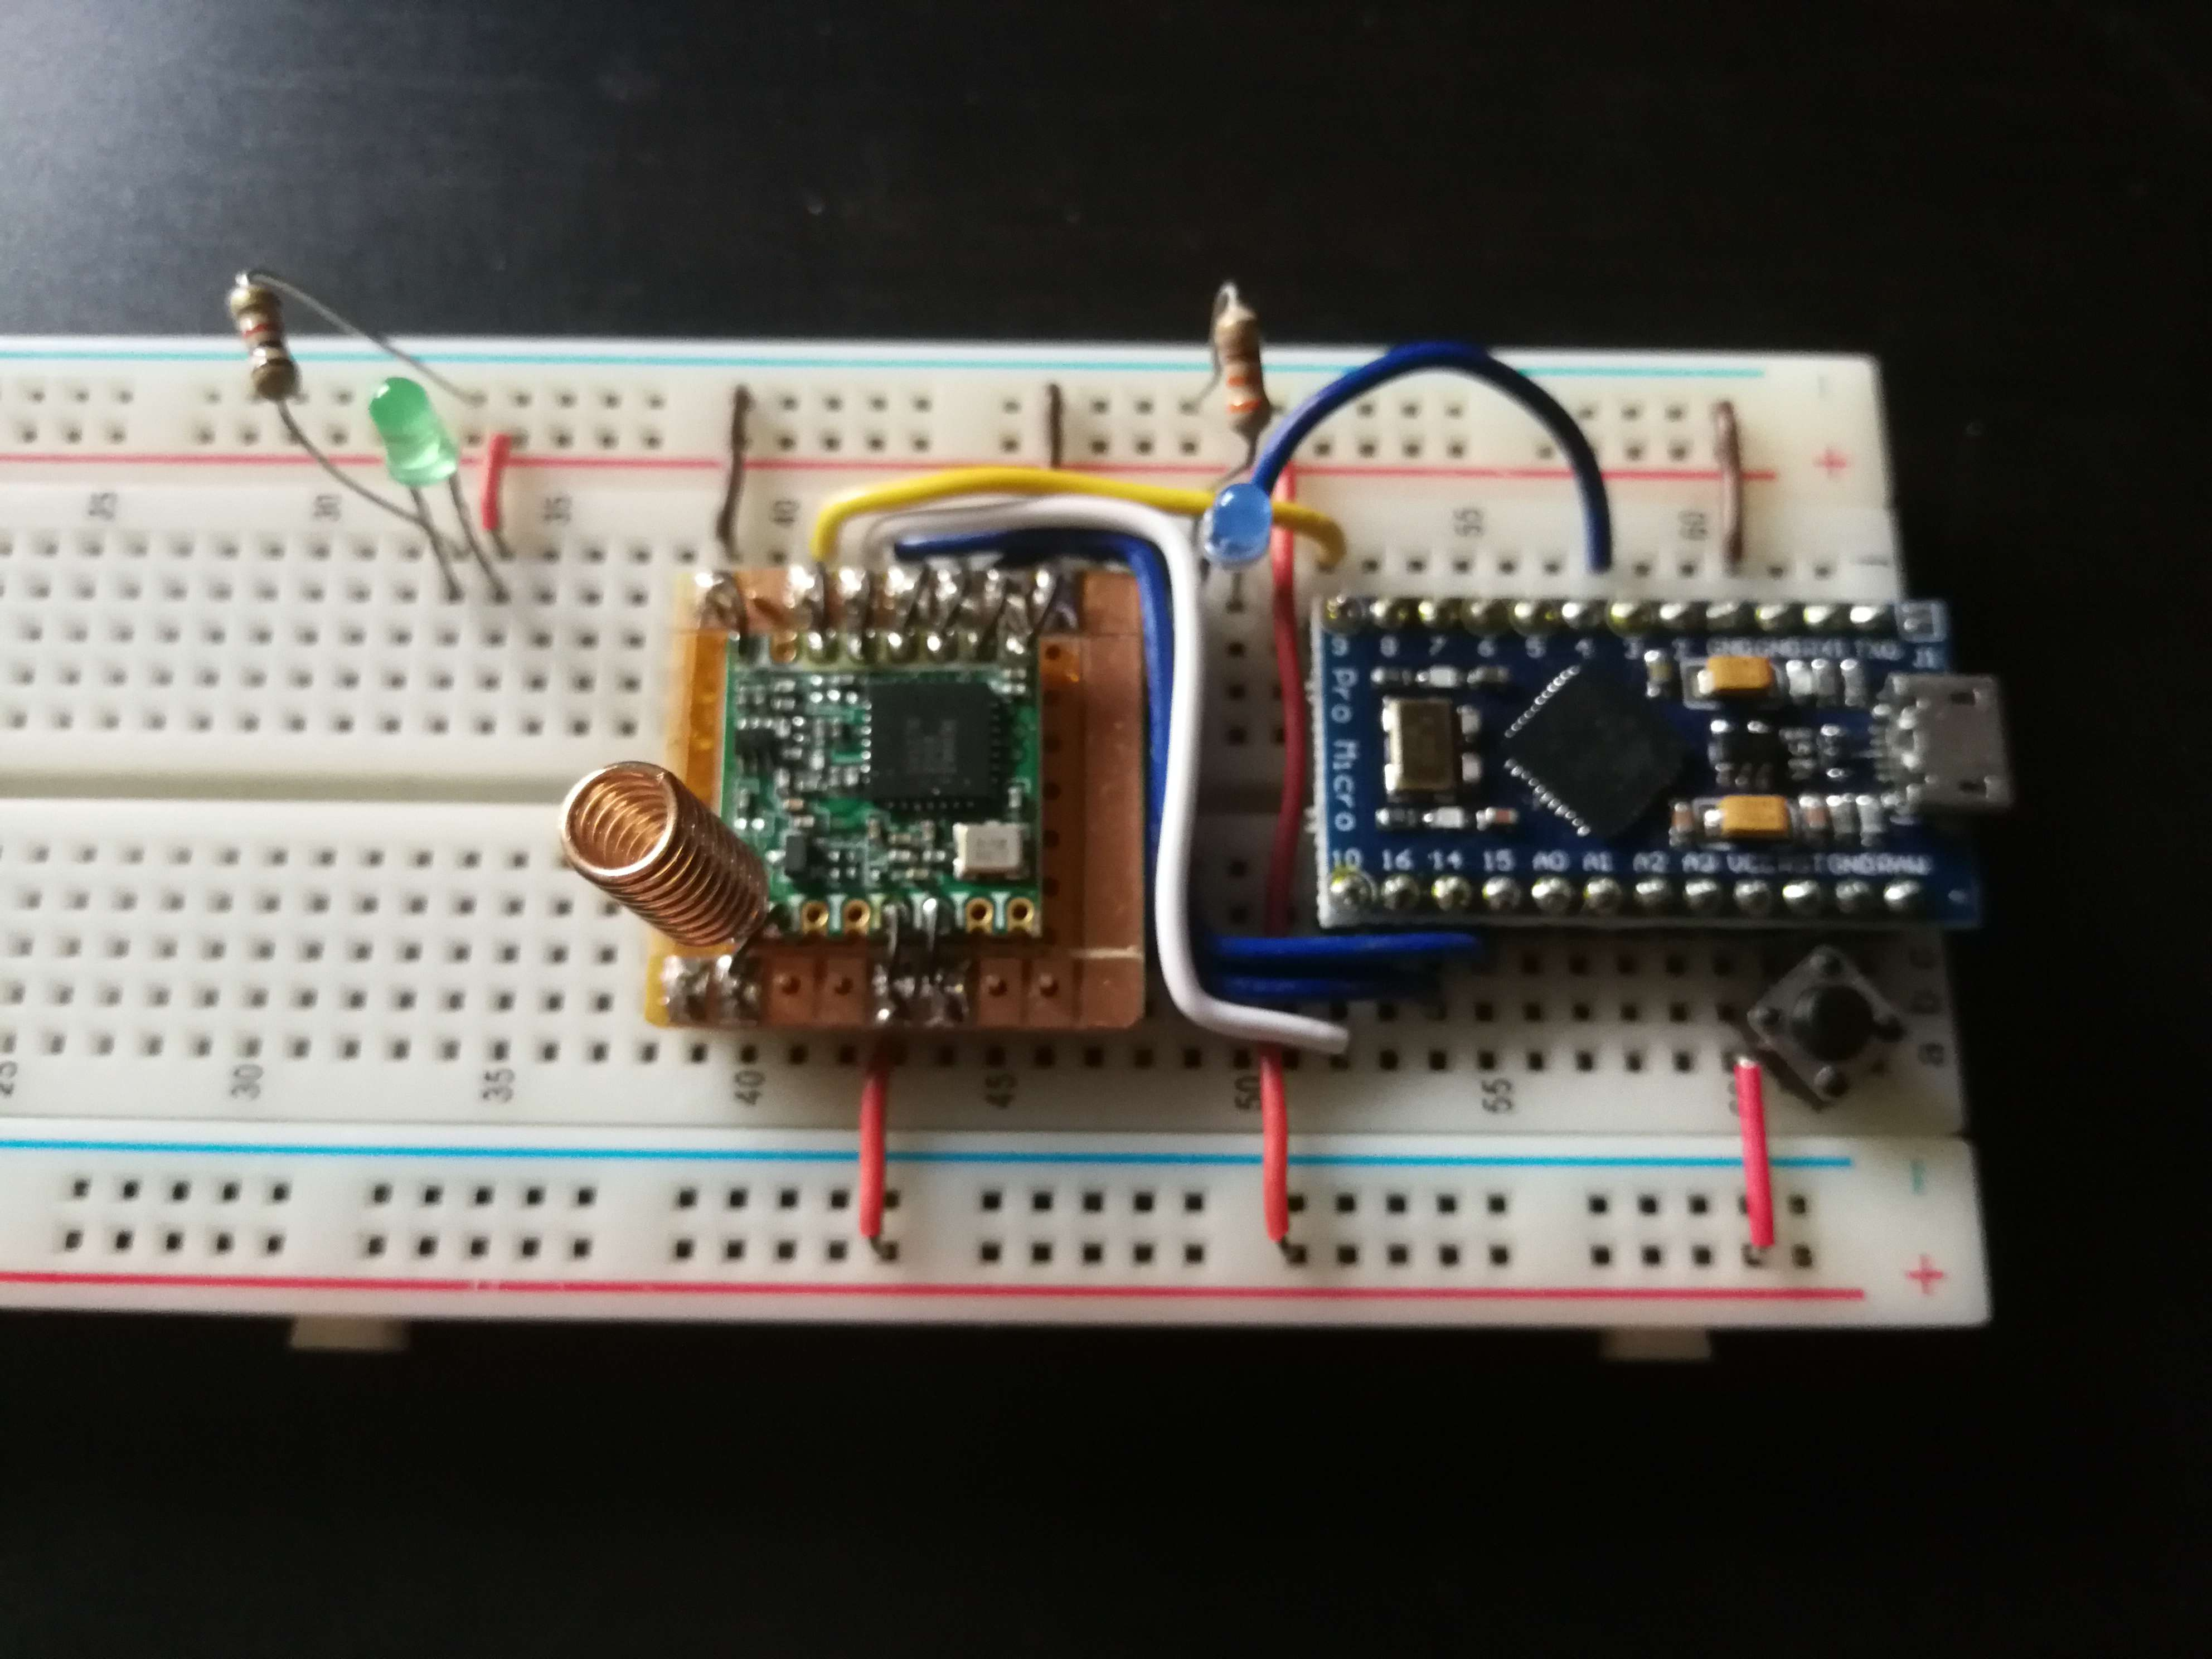
\includegraphics[scale=0.08]{images/arduino.png}
\caption{Un module Arduino}\label{term36}
\end{figure}

Sur la figure \ref{term36}, on peut voir que le module contient x. L'avantage principal de cet module est qu'il est possible de configurer une largeur de bande bien plus faible que les autres modules. Les modules rn2483 ou lopy ont une largeur de bande minimal de 125KHz, tanidis qu'avec l'arduino il possible de descendre jusqu'à x Khz. Pour rappel, une largeur de bande plus fiable permet un time on air plus grand, ce qui être utile pour analyser les signaux. 

\subsection{Logiciels}

Une fois les différents appareils choisis, il faut les accompagner avec les softwares adéquats. Ainsi il faut des logiciel d'analyse de signaux compatible avec les différents modules et radio logicielles.

\subsubsection{GQRX}

Le premier logiciel choisi est \textit{GQRX}. c'est un logiciel open source d'analyse de fréquence radio pour les SDR. Le fonctionnement du logiciel est assez direct, la figure \ref{term37} montre comment configurer simplement le logiciel. LA figure \ref{term331} demande de compléter les paramètres suivants:

\begin{itemize}
\item device. Il faut sélectionner la SDR dans la liste des appareils. Le \textit{Device String} fait référence à cet appareil dans gqrx.
\item Input rate. Le taux d'échantillonage capturé par la SDR, il apparait plus bas comme \textit{sample rate}.
\item Decimation. C'est un procédé qui permet de réduire le nombre d'échantillons géré par le logiciel, pour économiser des ressources.
\item Bandwidth. La largeur de bande supplémentaire que peut gérer la SDR.
\item \textit{Low Noise Block Local Oscillator (LNB LO)}. ce paramètre est spécifique à la réception satéllite et répresénte le frequency offset aplliqué par l'oscillateur locale dans un LNB downconverter.
\item l'audio output concerne la sortie sonnore du signal.
\end{itemize}

La figure \ref{term341} ajoute des paramètes pour le récepteur, c'est à dire pour l'interface de GQRX :

\begin{itemize}
\item frequency. La fréquence que l'on souhaite écouter.
\item Filter Width. Ce paramètre permet de changer la taille de la largeur de bande du filtre appliqué au signal.
\item Filter Shape. Contrairement au Filter Width ce n'est pas la taille mais la forme du filtre que l'on peut modifier.
\item Mode. Le mode de démodulation.
\item Automatic Gain Control (ACG). l'ACG ajuste le gain du récepteur pour maintenir un signal constant.
\item Squelch. C'est un trashold qui coupe la sortie sonore si il est franchi.
\item Noise blanker. C'est une fonctionnalité qui permet de rédure l'impact des interférence sur le signal.
\end{itemize}

\begin{figure}[h]
\centering
\begin{subfigure}{0.4\textwidth}
  \centering
  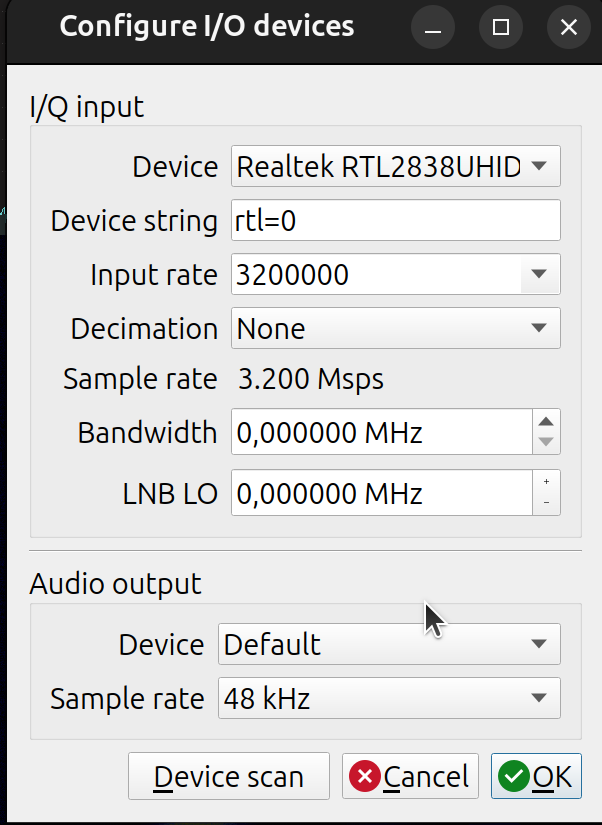
\includegraphics[width=\textwidth]{images/gqrx2.png}
  \caption{SDR input}
  \label{term331}
\end{subfigure}
\hspace{0.5cm} % Adjust the horizontal space between the subfigures
\begin{subfigure}{0.4\textwidth}
  \centering
  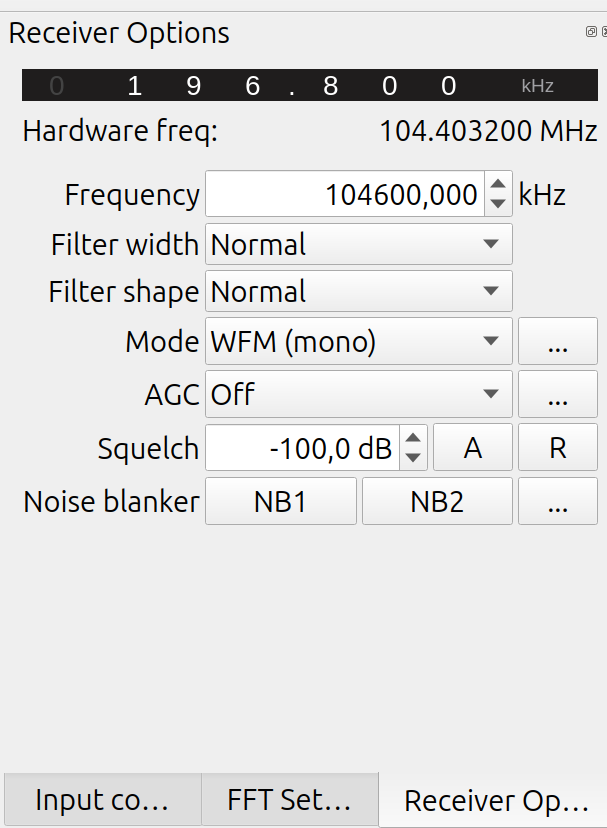
\includegraphics[width=\textwidth]{images/gqrx3.png}
  \caption{Receiver option}
  \label{term341}
\end{subfigure}
\caption{Configuration GQRX}
\label{term37}
\end{figure}

La figure montre un exemple de ce qu'on observe quand on écoute la fréquence radio de Classic21. GQRX affiche le signal reçu sous deux formes différentes : en spectre et en cascade.

\begin{figure}[h]
\centering

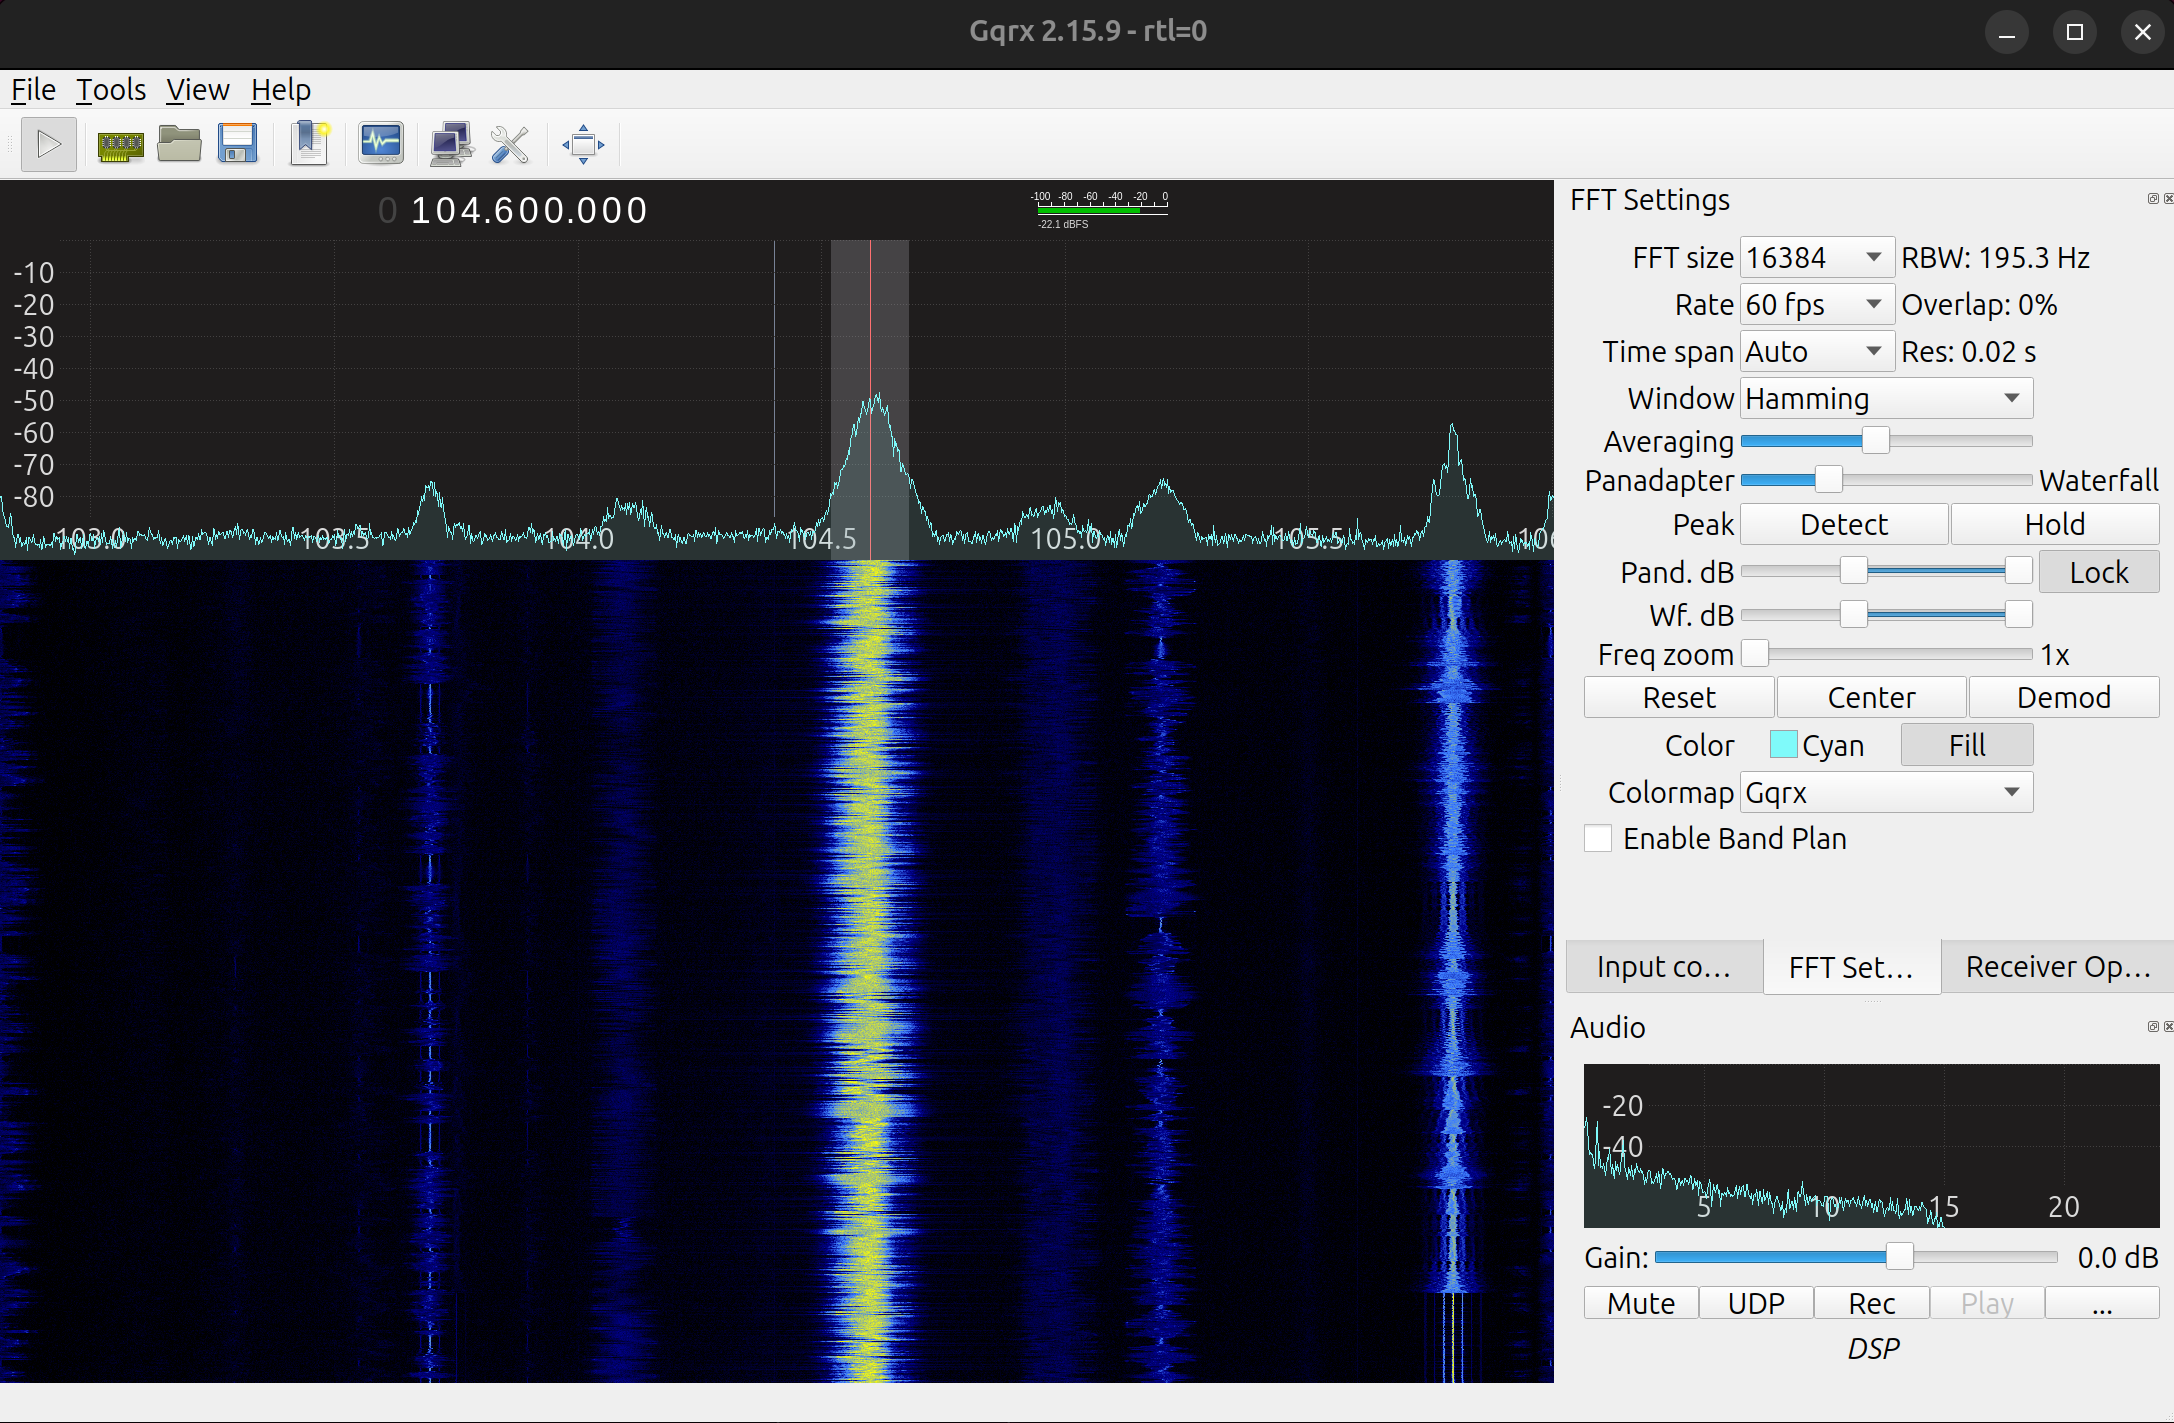
\includegraphics[scale=0.2]{images/gqrx1.png}
\caption{Réception de la station radio Classic21}\label{term38}
\end{figure}

L'affichage du spectre fournit une représentation graphique en temps réel du spectre RF sur une gamme de fréquences.
Il montre la puissance du signal de différentes fréquences sur une plage de fréquences spécifiée.
L'axe des x représente la fréquence, tandis que l'axe des y affiche la force du signal (mesurée en dB).

L'affichage en cascade est un spectrogramme qui visualise la force du signal au fil du temps.
Il montre une série d'instantanés de spectre empilés les uns sur les autres, où l'intensité de la couleur représente la force du signal.
Chaque ligne horizontale du tracé en cascade représente une vue du spectre capturée à un moment précis, créant ainsi un enregistrement historique de l'activité du signal.
L'axe vertical représente la fréquence et l'axe horizontal représente le temps.

Durant la réception du signal, il est possible de modifier l'affichage. A droite de l'affichage en spectre et en cascade sur la figure \ref{term38}, il y a différent paramètres :

Pour l'affichage en spectre, le paramètre \textit{Panadapter dB} fait référence à l'échelle verticale dans la vue du spectre. Il représente la force du signal des fréquences radio reçues affichées sur l'axe vertical du graphique du spectre. Le réglage du paramètre Panadapter dB modifie l’échelle verticale de la force du signal affichée dans la vue du spectre.

Pour l'affichage en cascade, le paramètre \textit{Waterfall dB} concerne l'intensité de la couleur ou l'ombrage des fréquences affichées dans le tracé en cascade.Le réglage du paramètre Waterfall dB modifie l'intensité utilisée pour afficher la force du signal dans le tracé en cascade, permettant ainsi d'ajuster le contraste ou la visibilité des signaux plus faibles ou plus forts.

Les paramètres suivants sont communs et affectes les deux affichages :

Le paramètres \textit{FFT size} détermine le nombre d'échantillons utilisé dans chaque calcul de FFT. Une valeur plus large donne un meilleure résolution, mais consome plus de ressources. La valeur est une puissance de deux pour des raisons d'éfficacité de calculs.

Le paramètre \textit{rate} détermine le taux de rafraichissement de l'affichage. Un taux relativement faible avec une taille de frame FFT élevé induit un effet d'overlap, c'est à dire que des frames consécutives partagent des échantillons, ce qui donne un affichage plus lisse du spectre.


\subsubsection{Universal radio hacker, URH}

Universal Radio Hacker est un logiciel open source similaire à GQRX. Son role principal est l'analyse de signaux radio. Au dela de l'écoute en temps réel, URH peut sauvegarder des signaux et lire des enregistrements à partir de fichiers. Les fichiers qu'URH peut interpréter ou enregistrer sont au format \textit{.complex}.  Ce format est utilisé pour pour sauvegarder les signaux sous forme d'échantillons \textit{I/Q (In phase / Quadrature)} Il existe plusieurs variantes de ce format supporté par URH :

\begin{itemize}
\item \textit{.complex (ou .complex64)}: c'est le format par défaut. LEs échantillons sont représenté par des float de 32bits pour les symboles I et Q respectivement (donc 64 bits au total)
 
\item  \textit{.complex16u}: la représentation en utilisant 2  entiers de 8 bits non signés pour I et Q.

\item  \textit{.complex16s}: la représentation en utilisant 2  entiers de 8 bits signés pour I et Q.

\item  \textit{.complex32u}: la représentation en utilisant 2  entiers de 16 bits non signés pour I et Q. 

\item  \textit{.complex32s}: la représentation en utilisant 2 entiers de 16 bits signés pour I et Q.
\end{itemize}

La figure \ref{term39} montre comment enregistrer un signal. Les paramètres à configurer sont similaires à GQRX (choix de la SDR, fréquence, taux d'échantillonage, largeur de bande et gain). Comme URH est le principal outils d'analyse pour ce travail, les analyse avec ce dernier sont détaillées dans la section \ref{signallora}.

\begin{figure}[h]
\centering

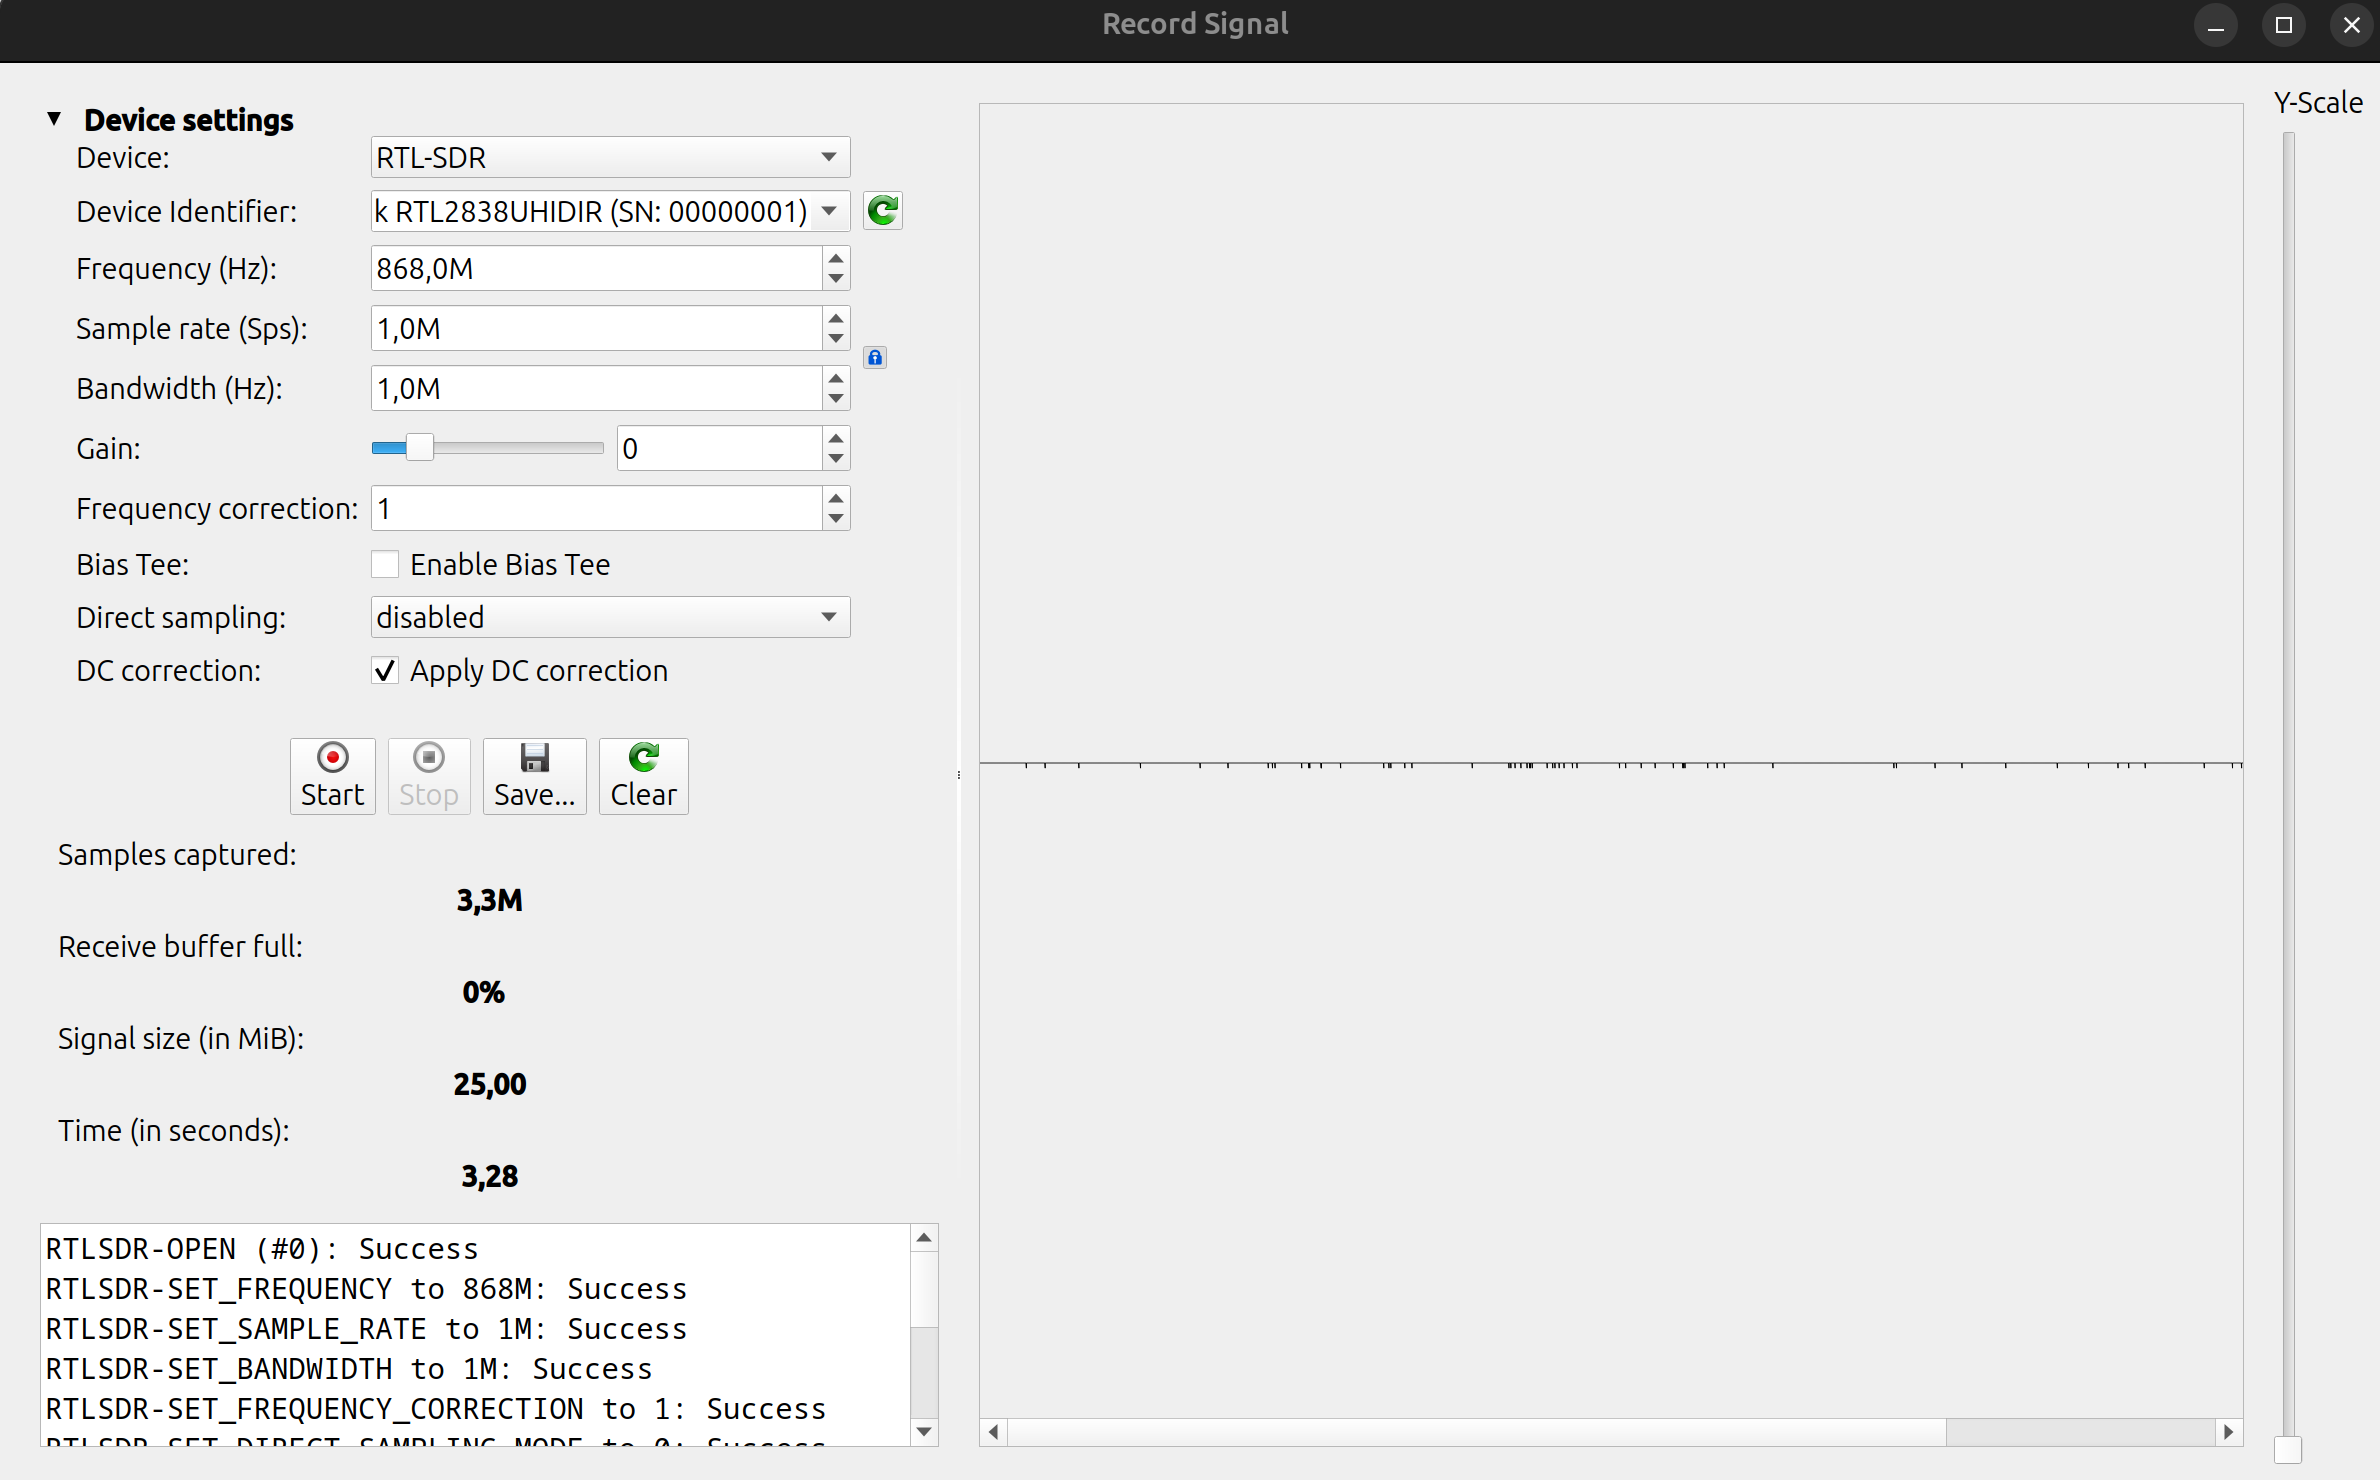
\includegraphics[scale=0.2]{images/urh1.png}
\caption{Enregistrement d'un signal avec URH}\label{term39}
\end{figure}


\subsubsection{Visual Studio Code}

L'environement de travail utilisé est Visual Studio Code (version 1.87.1). Cet IDE est open source et largement populaire ce qui permet un apprentissage pour des travaux spécifique très rapide via Internet. 

L'utilisiation de VSCode est motivé par son système d'extension, qui contient plusieurs extension qui permettent de manipuler directement les modules d'émission LoRa. Le module Lopy de Pycom est compatible avec VSCode via l'extension PyMakr.

GitHub est également intégré dans VSCode, ce qui permet de simplifier la mise en ligne du travail.

\subsubsection{IDE Arduino}

L'utilisation de l'IDE Arduino 2.2.1 est nécessaire pour la configuration du module Arduino décrit dans la section \ref{arduino}. L'IDE permet d'uploader le code  dans le module. Le code est disponible dans l'annexe.

\section{Librairie python}

Le choix du langage pour l'implémentation du travail est Python (version 3.11.4). Python donne l'accès à plusieurs librairie très pertinente pour le signal processing. Voici les principales librairies utilisées :

\begin{itemize}
\item Numpy. Cette librairie est fondamentale pour la gestion d'array. Elle contient également de nombreuse fonction et format mathématique utile au projet.
\item Matplotlib. Cette librairie permet d'effectuer des plots des données de manières simple et efficace.
\item Pyrtlsdr. La librairie PyRTLSDR est essentielle pour pouvoir manipuler la SDR R820T2. Il est possible de configurer la SDR sans devoir passer par un software tier comme GQRX ou URH grâce à cette librairie.
\item HackRf. L'équivalent de PyRTLSDR mais pour la SDR HackrF One.
\item datashader. Cette librairie permet la visualisation améliorée de grande quantité de données via l'ajout de gradient coloré.
\item serial. La manipulation des modules rn2483 est possible grave à la librairie serial.
\end{itemize}


\section{Géneration et réception d'un signal LoRa} \label{signallora}

dans un premier temps les signaux sont généré manuellement sans automatisation, le but étant de reconnaitre et d'analyser la structure d'un signal Lora. le premier signal est généra via le module rn2483. Via python, il est possible d'utiliser la librairie \textit{Serial} pour se connecter au port usb reliant le module à l'ordinateur. Ensuite, via les différentes commandes, on configure le module en modifiant les paramètres suivant : 

\begin{itemize}
\item la modulation, en LoRa.
\item la fréquence. 868MHz, la fréquence de la bande ISM , la bande d'émission en Europe.
\item la largeur de bande. Dans un premier but de visualiation, on souhaiterai que le message soit le plus long possible dans le temps pour pouvir l'observer facilement. Ainsi la largeur de bande choisie est de 125Khz, ce qui est la plus petite possible valeur que permet le module.
\item la puissance du module, au maximum (14W).
\item le spreading factor. Même raisonement que pour la largeur de bande, on souhaite que le \textit{time on air} soit le plus long possible, donc la valeur la plus grande possible est choisie (SF = 12)
\item le coding rate. Il y a 4 valeur possible:s 4/5, 4/6, 4/7 and 4/8. Cela signifie que tout les 4 bits seront codé par 4, 5, 6, 7 ou 8 bits de transmissions en fonction de cette valeur. Plus la valeur st faible (la plus faible étant 4/8), plus le time on air sera élevé, car cela prend plus de temps pour transmettre le message.
\end{itemize}

Les commandes relatives à la configuration sont disponibles en annexes.
Une fois que le module est configurer, il faut paramètrer le recpeteur, la radio logicielle. La librairie pyrtlsdr permet de pouvoir configurer le récepteur, elle sera utlisée pour les expérmientations dans la section 3.4. Dans un premier temps, les logiciels comme gqrx ou urh permettent également de pouvoir configurer le récepteur. Leur utilisation a déja été décrite dans la section 3.1.3. Les paramètres à configurer sont les suivant : 

\begin{itemize}
\item la fréquence. La fréquece d'écoute. Idéalement la même fréquence de celle de l'émetteur (868MHz). Cependant celle ci sera légèrement décalée pour contrer un effet
\item le taux d'échantillonage. Il est possible de choisir la quantitté d'échantillons traitée chaque seconde. Un taux plus élevé donnera un signal plus complet. Le taux minimal ne doit jamais être inférieur à deux fois la largeur de bande. (Théorème de nyquist shannon : fe > 2fmax)
\item le gain. Dépendant de la qualité du signal il peut être nécessaire d'ajouter du gain, c'est à dire d'amplifier la force du signal. Un gain trop élevé peut saturer le signal, quand l'amplitude dépasse la portée du récepteur.
\end{itemize}

Une fois l'émetteur et le récepteur configuré, il est maintenant possible de visualiser des signaux Lora.

\subsection{analyse du signal}

affichage du signal capturé, d'abords sous forme analogique, puis en spectrogramme.
Décomposition du signal, on observe des "chirps". En analogique, augmentation de la fréquence (unchirp) et diminution de la fréquence (downchirp). En spectrogramme, augmentation est plus visuelle encore, on voit de manière net les chirps.

Dans le signal, on reconnait donc le préambule du signal composé de 10 upchirps et 2 downchirps (selon la théorie).

Attention, la fréquence d'écoute des sdr ne doit pas être exactement à 868Mhz. En effet, voilà à quoi ressemble si la fréquence d'écout est la même que la fréquence d'émission. Il faut prendre en compte la largeur de bande du signal, dans le cas ou le singal a une largeur de bande de 125KHz, il faut décaler la fréquence d'écoute pour recentrer le signal, ainsi on évite d'avoir des fréquence qui sont interprétée comme "négatives" par URH. Dans la figure, la fréquence est décalé de 125/2 soit 867,935Mhz.

\subsection{automatisation du signal et preprocessing}

Dans un second temps, besoin d'automatiser la génération et l'enregistrement des signaux afin de pouvoir travailler avec un grand nombre d'échantillons. La librairie python pytlsdr permet de ne pas devoir passer par un logiciel comme urh pour sauvegarder les échantillons. La méthode d'enregistrement est la suivate :

\begin{itemize}
\item d'abords, configurer la module et la rtlsdr avec les différent paramètre
\item ensuite l'antenne commence a enregistrer. L'émetteur est informé que la radio logiciel est en écoute et envoie un signal. 
\item dès que la radio reçoit le signal, elle informe l'émetteur de se mettre en attente car le preprocessing commence.
\item Le signal reçu est découpé pour ne conserver que le preambule, et puis enregistrer dans un fichier.
\item dès que l'enregistrement est terminé, le cycle recommence.
\end{itemize}

la code source est disponible en annexe.


\section{Méthode "Constellation traces"}

objectif, identification du device via son frequecy offset.

selon l'article (citer article), possible de performer la méthode soit uniquement sur le  préambule, soit sur l'intégralité du singal. 

idée: le received singal contient le baseband singal ainsi qu'un rotation factor instable. pour pouvoir recover cette partie du signal, besoin d'effctuer une opération différentielle suivante : $$ x(t) . x(t+n) e -j2\pi on $$
apparation d'un nouveau rotation factor, mais stable. Besoin de trouver deux inconnue,\textit{delta f} et \textit{n}. n est le differential interval. il se calcule de la manière suivante : $$ Rs = BW / 2sf $$ 
$$ N = fs / Rs $$

delta f est la difference entre le transmitter carrier frequency et le receiver carrier frequecy.

application : récupérer les samples I/Q du signal n ayant au préalable "clean" le signal. utilisation d'un gradiant pour observer la dentsité sur le plot. noramlement des zones plus denses apparaissent.
coloration : utilisation de la librairie data shader. 


clustering, le but de conserver les parties les plus dense (95pourcent du point le plus dense) plot avec les différents appareils.
librairie panda et numpy. découpage en zones (bins?) sous forme d'une grille, calcul de nobre de points dans chaque zone, la zone avec le plus grand nombre de point sers de maximum. 
